\documentclass{article}

\usepackage[top=0.60in, bottom=0.60in, left=0.5in, right=0.5in]{geometry} 
\usepackage{ulem}			% For strikeout command \sout
\usepackage{circuitikz}
\usepackage{tikzducks}			% for ducks
\usetikzlibrary{snakes, decorations}
\usepackage{enumerate}

\begin{document}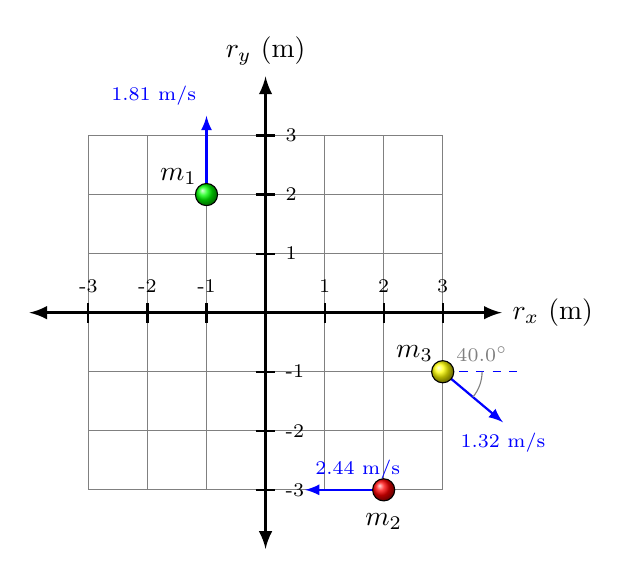
\begin{tikzpicture}[> = latex]

	% Definition
	
	\def\L{0.75};

	% The grid
	
	\draw [thin, gray, step = \L cm] (-3 * \L, -3 * \L) grid (3 * \L, 3 * \L);
	
	% Axes
	
	\begin{scope}[<->, very thick]
	
		\draw (-4 * \L, 0) -- (4 * \L, 0) node [right] {$r_x$ (m)};
		\draw (0, -4 * \L) -- (0, 4 * \L) node [above] {$r_y$ (m)};
		
	\end{scope}
	
	\foreach \n in {-3, -2, -1, 1, 2, 3}
	{
		\draw [thick] (\L* \n, -0.125) -- (\L * \n, 0.125) node [above, font = \scriptsize] {\n};
		\draw [thick] (-0.125, \L * \n) -- (0.125, \L * \n) node [right, font = \scriptsize] {\n};
	}
	
	% Objects w/masses, velocities
	
	\draw [->, thick, blue] (-\L, 2 * \L) -- ++ (0, 1) node [above left, font = \scriptsize] {1.81 m/s};
	\draw [ball color = green] (-\L, 2 * \L) circle (4 pt) node [above left] {$m_1$};
	
	\draw [->, thick, blue] (2 * \L, -3 * \L) -- ++ (-1, 0) node [above right, font = \scriptsize] {2.44 m/s};
	\draw [ball color = red] (2 * \L, -3 * \L) circle (4 pt) node [below = 0.5 em] {$m_2$};
	
	\draw [->, thick, blue] (3 * \L, -\L) -- ++ (-40 : 1) node [below, font = \scriptsize] {1.32 m/s};
	\draw [blue, dashed] (3 * \L, -\L) -- ++ (1, 0);
	\draw [gray] (3 * \L + 0.5, -\L) node [above, font = \scriptsize] {$40.0^\circ$} arc (0 : -40 : 0.5);
	\draw [ball color = yellow] (3 * \L, -\L) circle (4 pt) node [above left] {$m_3$};

\end{tikzpicture}

\vspace{1em}

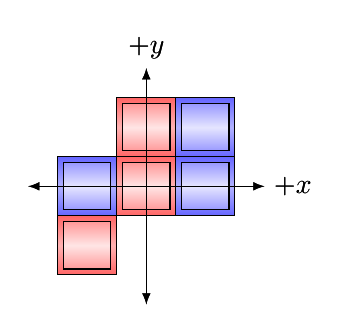
\begin{tikzpicture}[> = latex]

	% Definition
	
	\def\L{0.75};
	
	% Coordinate axes
	
	\draw [<->] (-2 * \L, 0) -- (2 * \L, 0) node [right] {$+x$};
	\draw [<->] (0, -2 * \L) -- (0, 2 * \L) node [above] {$+y$};
	
	% Tiles making up shape
	
	\foreach \x/\y/\col in {0/0/red, 1/0/blue, -1/-1/red, 0/1/red, -1/0/blue, 1/1/blue}
	{
		\draw [top color = \col!60, bottom color = \col!60, middle color = \col!30] ({(\x - 0.5) * \L}, {(\y - 0.5) * \L}) rectangle ({(\x + 0.5) * \L}, {(\y + 0.5) * \L});
		\draw [top color = \col!40, bottom color = \col!40, middle color = \col!10] ({(\x - 0.4) * \L}, {(\y - 0.4) * \L}) rectangle ({(\x + 0.4) * \L}, {(\y + 0.4) * \L});
	}
	
	% Coordinate axes
	
	\draw [<->] (-2 * \L, 0) -- (2 * \L, 0) node [right] {$+x$};
	\draw [<->] (0, -2 * \L) -- (0, 2 * \L) node [above] {$+y$};

\end{tikzpicture}

\vspace{1em}

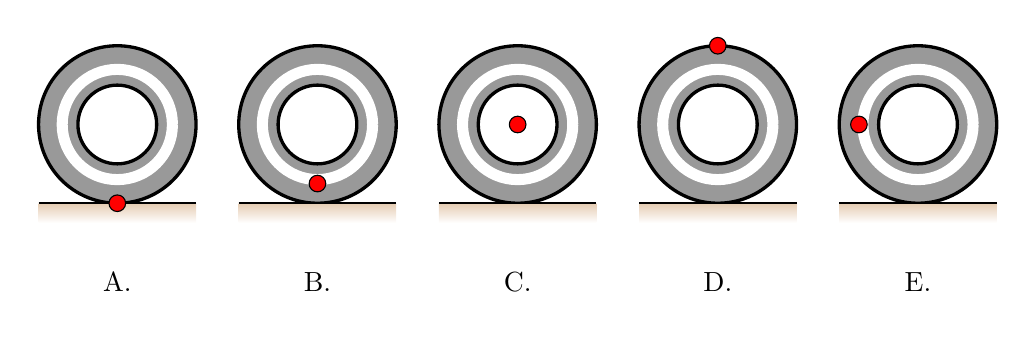
\begin{tikzpicture}
\matrix[column sep = 0.5 cm]{

	% Tire
	
	\draw [very thick, fill = gray!80] (1, 1) arc (0 : 360 : 1)
		(0.5, 1) arc (360 : 0 : 0.5);
		
	\draw [line width = 4 pt, white] (0.7, 1) arc (0 : 360 : 0.7);

	% Ground
	
	\draw [top color = brown!40, bottom color = white, draw = none] (-1, 0) rectangle (1, -0.25);
	\draw [thick] (-1, 0) -- (1, 0);
	
	% CM mark
	
	\draw [fill = red] (0, 0) circle (3 pt);
	
	% Label
	
	\node at (0, -1) {A.};
	
&

	% Tire
	
	\draw [very thick, fill = gray!80] (1, 1) arc (0 : 360 : 1)
		(0.5, 1) arc (360 : 0 : 0.5);
		
	\draw [line width = 4 pt, white] (0.7, 1) arc (0 : 360 : 0.7);

	% Ground
	
	\draw [top color = brown!40, bottom color = white, draw = none] (-1, 0) rectangle (1, -0.25);
	\draw [thick] (-1, 0) -- (1, 0);
	
	% CM mark
	
	\draw [fill = red] (0, 0.25) circle (3 pt);
	
	% Label
	
	\node at (0, -1) {B.};
	
&

	% Tire
	
	\draw [very thick, fill = gray!80] (1, 1) arc (0 : 360 : 1)
		(0.5, 1) arc (360 : 0 : 0.5);
		
	\draw [line width = 4 pt, white] (0.7, 1) arc (0 : 360 : 0.7);

	% Ground
	
	\draw [top color = brown!40, bottom color = white, draw = none] (-1, 0) rectangle (1, -0.25);
	\draw [thick] (-1, 0) -- (1, 0);
	
	% CM mark
	
	\draw [fill = red] (0, 1) circle (3 pt);
	
	% Label
	
	\node at (0, -1) {C.};
	
&

	% Tire
	
	\draw [very thick, fill = gray!80] (1, 1) arc (0 : 360 : 1)
		(0.5, 1) arc (360 : 0 : 0.5);
		
	\draw [line width = 4 pt, white] (0.7, 1) arc (0 : 360 : 0.7);

	% Ground
	
	\draw [top color = brown!40, bottom color = white, draw = none] (-1, 0) rectangle (1, -0.25);
	\draw [thick] (-1, 0) -- (1, 0);
	
	% CM mark
	
	\draw [fill = red] (0, 2) circle (3 pt);
	
	% Label
	
	\node at (0, -1) {D.};
	
&

	% Tire
	
	\draw [very thick, fill = gray!80] (1, 1) arc (0 : 360 : 1)
		(0.5, 1) arc (360 : 0 : 0.5);
		
	\draw [line width = 4 pt, white] (0.7, 1) arc (0 : 360 : 0.7);

	% Ground
	
	\draw [top color = brown!40, bottom color = white, draw = none] (-1, 0) rectangle (1, -0.25);
	\draw [thick] (-1, 0) -- (1, 0);
	
	% CM mark
	
	\draw [fill = red] (-0.75, 1) circle (3 pt);
	
	% Label
	
	\node at (0, -1) {E.};

\\	
};

\end{tikzpicture}

\vspace{1em}

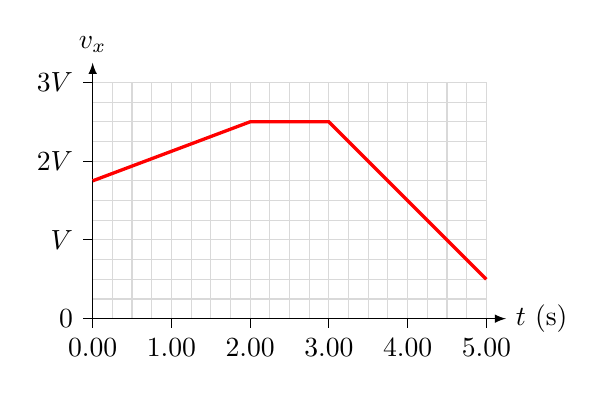
\begin{tikzpicture}[> = latex]

	% Axes
	
	\draw [thin, gray!30, step = 0.25 cm] (0, 0) grid (5, 3);
	\draw [<->] (0, 3.25) node [above] {$v_x$} -- (0, 0) -- (5.25, 0) node [right] {$t$ (s)};
	
	% Axis labels
	
	\draw (0, 0) -- (-0.125, 0) node [left] {0};
	\draw (0, 1) -- (-0.125, 1) node [left] {$V$};
	\draw (0, 2) -- (-0.125, 2) node [left] {$2V$};
	\draw (0, 3) -- (-0.125, 3) node [left] {$3V$};
	
	\foreach \x in {0.00, 1.00, 2.00, 3.00, 4.00, 5.00}
		\draw (\x, 0) -- (\x, -0.125) node [below] {\x};
	
	% Curve
	
	\draw [red, very thick] (0, 1.75) -- (2, 2.5) -- (3, 2.5) -- (5, 0.5);

\end{tikzpicture}

\vspace{1em}

\begin{tabular}{lc}
\begin{minipage}{3cm}
\begin{enumerate}[A.]

	\item 1, 2, 2

	\item 1, 2, 3

	\item 2, 3, 3

	\item 2, 3, 4

	\item 3, 3, 3

\end{enumerate}
\end{minipage}
&
\begin{minipage}{5cm}
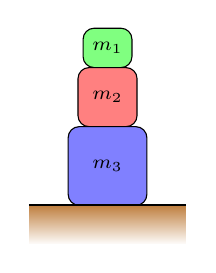
\begin{tikzpicture}[every node/.style = {rectangle, rounded corners, draw = black}, font = \scriptsize]

	\node [minimum size = 0.5 cm, fill = green!50] at (0, 1.5) {$m_1$};
	\node [minimum size = 0.75 cm, fill = red!50] at (0, 0.875) {$m_2$};
	\node [minimum size = 1 cm, fill = blue!50] at (0, 0) {$m_3$};
	
	\draw [bottom color = white, top color = brown, draw = white] (-1, -1) rectangle (1, -0.5);
	\draw [thick] (-1, -0.5) -- (1, -0.5);

\end{tikzpicture}
\end{minipage}
\\
\end{tabular}

\begin{enumerate}[A.]

	\item 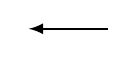
\begin{tikzpicture}\draw [> = latex, thick, ->] (0, 0) -- (-1, 0);\end{tikzpicture}

	\item 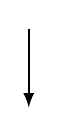
\begin{tikzpicture}\draw [> = latex, thick, ->] (0, 0) -- (0, -1);\end{tikzpicture}

	\item 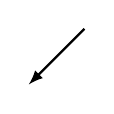
\begin{tikzpicture}\draw [> = latex, thick, ->] (0, 0) -- (225 : 1);\end{tikzpicture}

	\item 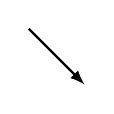
\begin{tikzpicture}\draw [> = latex, thick, ->] (0, 0) -- (315 : 1);\end{tikzpicture}

	\item zero ${\vec F}$

\end{enumerate}

\vspace{1em}

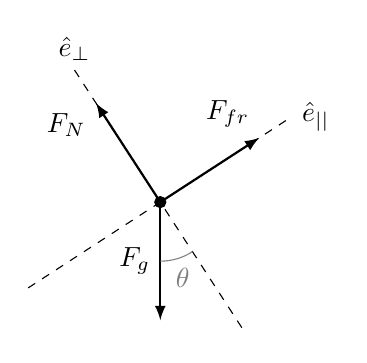
\begin{tikzpicture}[> = latex]

	% Define the ramp angle
	
	\def\Q{33}
	
	% The dot
	
	\filldraw (0, 0) circle (2 pt);
	
	% Coordinate axes
	
	\draw [dashed] (180 + \Q : 2) -- (\Q : 2) node [right] {${\hat e}_{||}$};
	\draw [dashed] (90 + \Q : 2) node [above] {${\hat e}_\perp$} -- (270 + \Q : 2);
	
	% Three forces on child
	
	\begin{scope}[->, thick]
	
		\draw (0, 0) -- (90 + \Q: 1.5) node [below left] {$F_N$};
		\draw (0, 0) -- node [left] {$F_g$} (270 : 1.5);
		\draw (0, 0) -- (\Q : 1.5) node [above left] {$F_{fr}$};
		
	\end{scope}
	
	% Angle indicator for force F_g
	
	\draw [gray] (0, -0.75) arc (270 : 270 + \Q: 0.75);
	\node [gray] at ({270 + 0.5 * \Q} : 1) {$\theta$};
		
\end{tikzpicture}

\vspace{1em}

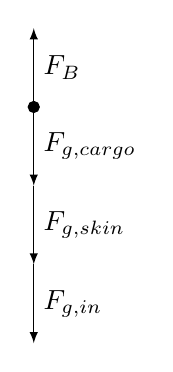
\begin{tikzpicture}[> = latex]
	
	% The dot
	
	\filldraw (0, 0) circle (2 pt);

	% Forces
	
	\begin{scope}[->]
	
		\draw (0, 0) -- node [right] {$F_B$} (0, 1);
		\draw (0, 0) -- node [right] {$F_{g, cargo}$} (0, -1);
		\draw (0, -1) -- node [right] {$F_{g, skin}$} (0, -2);
		\draw (0, -2) -- node [right]{$F_{g, in}$} (0, -3);
		
	\end{scope}

\end{tikzpicture}

\vspace{1em}

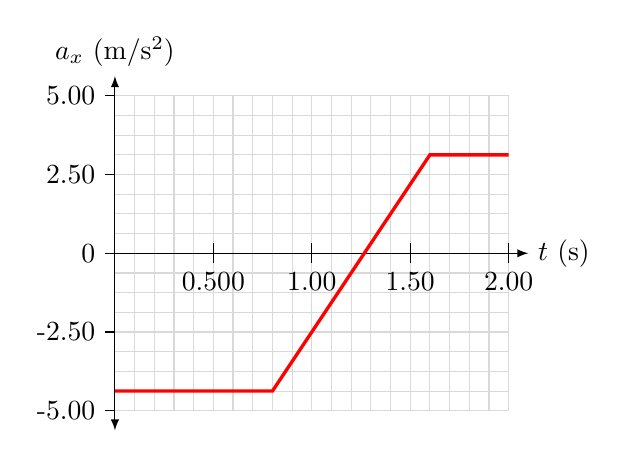
\begin{tikzpicture}[> = latex]

	% Axes + grid
	
	\draw [thin, gray!30, step = 0.25 cm] (0, -2) grid (5, 2);
	
	\draw [<->] (0, -2.25) -- (0, 2.25) node [above] {$a_x$ (m/s$^2$)};
	\draw [->] (0, 0) -- (5.25, 0) node [right] {$t$ (s)};
	
	% Axis ticks
	
	\foreach \x in {0.500, 1.00, 1.50, 2.00}
		\draw (2.5 * \x, 0.125) -- (2.5 * \x, -0.125) node [below] {\x};
	
	\foreach \y in {-5.00, -2.50, 0, 2.50, 5.00}
		\draw (0, 0.4 * \y) -- (-0.125, 0.4 * \y) node [left] {\y};
		
	% Curve
	
	\draw [red, very thick] (0, -1.75) -- (2, -1.75) -- (4, 1.25) -- (5, 1.25);

\end{tikzpicture}

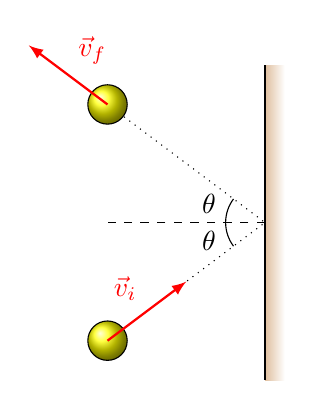
\begin{tikzpicture}[> = latex]

	% Wall + normal
	
	\draw [left color = brown!50, right color = white, draw = none] (0, -2) rectangle (0.25, 2);
	\draw [thick] (0, -2) -- (0, 2);
	
	\draw [dashed] (0, 0) -- (-2, 0);
	
	% Ball + its motion
	
	\draw [dotted] (-2, -1.5) -- (0, 0) -- (-2, 1.5);
	
	\draw [ball color = yellow] (-2, -1.5) circle (0.25 cm);
	\draw [ball color = yellow] (-2, 1.5) circle (0.25 cm);
	
	% Velocity vectors
	
	\begin{scope}[thick, red, ->]
	
		\draw (-2, -1.5) -- node [above left] {${\vec v}_i$} (-1, -0.75);
		\draw (-2, 1.5) -- node [above right] {${\vec v}_f$} (-3, 2.25);
	
	\end{scope}
	
	% Angle indicators
	
	\draw (-0.5, 0) arc (180 : {180 + atan(0.75)} : 0.5);
	\node at ({180 + 0.5 * atan(0.75)} : 0.75) {$\theta$};
	
	\draw (-0.5, 0) arc (180 : {180 - atan(0.75)} : 0.5);
	\node at ({180 - 0.5 * atan(0.75)} : 0.75) {$\theta$};

\end{tikzpicture}

\vspace{1em}

\begin{tabular}{cl}
\begin{minipage}{9cm}
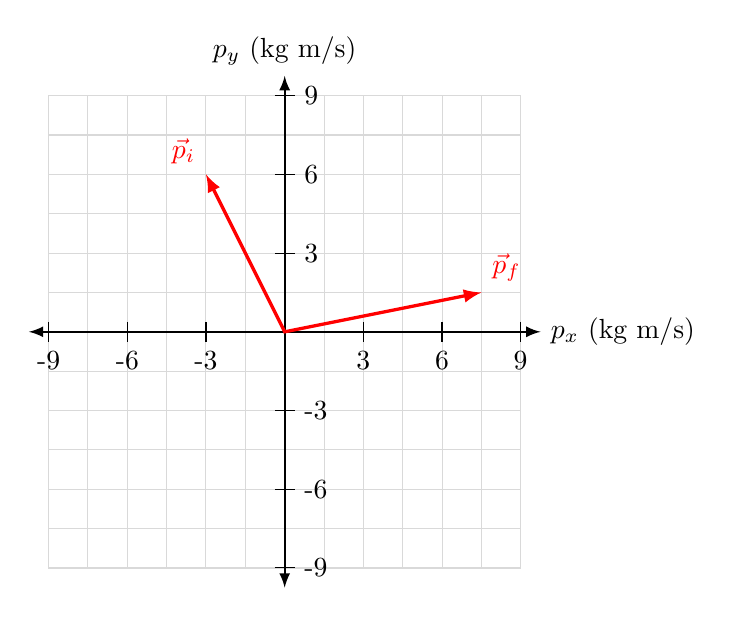
\begin{tikzpicture}[> = latex]

	% Grid
	
	\draw [thin, gray!30, step = 0.5 cm] (-3, -3) grid (3, 3);

	% Axes
	
	\begin{scope}[<->, thick]
	
		\draw (-3.25, 0) -- (3.25, 0) node [right] {$p_x$ (kg m/s)};
		\draw (0, -3.25) -- (0, 3.25) node [above] {$p_y$ (kg m/s)};
		
	\end{scope}
	
	% Vectors
	
	\draw [very thick, red, <->] (-1, 2) node [above left] {${\vec p}_i$} -- (0, 0) -- (2.5, 0.5) node [above right] {${\vec p}_f$};
	
	% Tick marks
	
	\foreach \n in {-9, -6, -3, 3, 6, 9}
	{
		\draw (0.333 * \n, 0.125) -- (0.333 * \n, -0.125) node [below] {\n};
		\draw (-0.125, 0.333 * \n) -- (0.125, 0.333 * \n) node [right] {\n};
	}

\end{tikzpicture}
\end{minipage}
&
\begin{minipage}{8cm}
\begin{enumerate}[A.]

	\item $(-3.50 \textrm{ kg m/s}) {\hat x} + (1.50 \textrm{ kg m/s}) {\hat y}$
	\item $(-3.00 \textrm{ kg m/s}) {\hat x} + (6.00 \textrm{ kg m/s}) {\hat y}$
	\item $(3.50 \textrm{ kg m/s}) {\hat x} + (-1.50 \textrm{ kg m/s}) {\hat y}$
	\item $(7.50 \textrm{ kg m/s}) {\hat x} + (1.50 \textrm{ kg m/s}) {\hat y}$
	\item $(10.5 \textrm{ kg m/s}) {\hat x} + (-4.50 \textrm{ kg m/s}) {\hat y}$

\end{enumerate}
\end{minipage}
\\
\end{tabular}

\vspace{1em}

\begin{tikzpicture}[> = latex]
\matrix[column sep = 0.25 cm]{

	% Axes
	
	\draw [<->] (0, -1) -- (0, 1) node [above] {$a_y$};
	\draw [->] (0, 0) -- (2, 0) node [right] {$t$};
	
	% Curve
	
	\draw [very thick, red] (0, -0.75) -- (2, -0.75);
	
	% Label
	
	\node at (1, -1.5) {A.};

&

	% Axes
	
	\draw [<->] (0, -1) -- (0, 1) node [above] {$a_y$};
	\draw [->] (0, 0) -- (2, 0) node [right] {$t$};
	
	% Curve
	
	\draw [very thick, red] plot [variable = \x, domain = 0 : 1.75, samples = 100] (\x, {-0.75 + 0.75 / (1 + exp(-5 * \x + 4))});
	
	% Label
	
	\node at (1, -1.5) {B.};

&

	% Axes
	
	\draw [<->] (0, -1) -- (0, 1) node [above] {$a_y$};
	\draw [->] (0, 0) -- (2, 0) node [right] {$t$};
	
	% Curve
	
	\draw [very thick, red] (0, -0.75) parabola [bend at end] (1.75, 0);
	
	% Label
	
	\node at (1, -1.5) {C.};

&

	% Axes
	
	\draw [<->] (0, -1) -- (0, 1) node [above] {$a_y$};
	\draw [->] (0, 0) -- (2, 0) node [right] {$t$};
	
	% Curve
	
	\draw [very thick, red] (0, -0.5) parabola (2, -1);
	
	% Label
	
	\node at (1, -1.5) {D.};

&

	% Axes
	
	\draw [<->] (0, -1) -- (0, 1) node [above] {$a_y$};
	\draw [->] (0, 0) -- (2, 0) node [right] {$t$};
	
	% Curve
	
	\draw [very thick, red] (0, -0.75) -- (1.75, 0);
	
	% Label
	
	\node at (1, -1.5) {E.};

\\
};

\end{tikzpicture}

\vspace{1em}

\begin{tikzpicture}[> = latex]
\matrix[column sep = 0.25 cm]{

	% Axes
	
	\draw [<->] (0, 2.25) node [above] {$r_y$} -- (0, 0) -- (2.25, 0) node [right] {$t$};
	
	% Curve
	
	\draw [very thick, red] plot [variable = \x, domain = 0 : 2, samples = 100] (\x, {2 * exp(-4 * \x)});
	
	% Label
	
	\node at (1, -1.5) {A.};

&

	% Axes
	
	\draw [<->] (0, 2.25) node [above] {$r_y$} -- (0, 0) -- (2.25, 0) node [right] {$t$};
	
	% Curve
	
	\draw [very thick, red] (0, 2) parabola [bend at end] (2, 0);
	
	% Label
	
	\node at (1, -1.5) {B.};

&

	% Axes
	
	\draw [<->] (0, 2.25) node [above] {$r_y$} -- (0, 0) -- (2.25, 0) node [right] {$t$};
	
	% Curve
	
	\draw [very thick, red] (0, 2) -- (2, 0);
	
	% Label
	
	\node at (1, -1.5) {C.};

&

	% Axes
	
	\draw [<->] (0, 2.25) node [above] {$r_y$} -- (0, 0) -- (2.25, 0) node [right] {$t$};
	
	% Curve
	
	\draw [very thick, red] (0, 2) parabola (2, 0);
	
	% Label
	
	\node at (1, -1.5) {D.};

&

	% Axes
	
	\draw [<->] (0, 2.25) node [above] {$r_y$} -- (0, 0) -- (2.25, 0) node [right] {$t$};
	
	% Curve
	
	\draw [very thick, red] plot [variable = \x, domain = 0 : 2, samples = 100] (\x, {2 * (1 - exp(-4 * (2 - \x)))});
	
	% Label
	
	\node at (1, -1.5) {E.};

\\
};

\end{tikzpicture}

\vspace{1em}

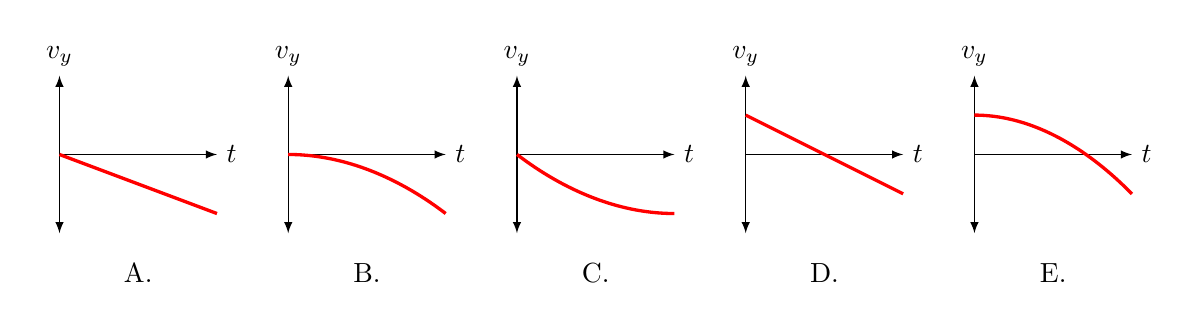
\begin{tikzpicture}[> = latex]
\matrix[column sep = 0.25 cm]{

	% Axes
	
	\draw [<->] (0, -1) -- (0, 1) node [above] {$v_y$};
	\draw [->] (0, 0) -- (2, 0) node [right] {$t$};
	
	% Curve
	
	\draw [very thick, red] (0, 0) -- (2, -0.75);
	
	% Label
	
	\node at (1, -1.5) {A.};

&

	% Axes
	
	\draw [<->] (0, -1) -- (0, 1) node [above] {$v_y$};
	\draw [->] (0, 0) -- (2, 0) node [right] {$t$};
	
	% Curve
	
	\draw [very thick, red] (0, 0) parabola (2, -0.75);
	
	% Label
	
	\node at (1, -1.5) {B.};

&

	% Axes
	
	\draw [<->] (0, -1) -- (0, 1) node [above] {$v_y$};
	\draw [->] (0, 0) -- (2, 0) node [right] {$t$};
	
	% Curve
	
	\draw [very thick, red] (0, 0) parabola [bend at end] (2, -0.75);
	
	% Label
	
	\node at (1, -1.5) {C.};

&

	% Axes
	
	\draw [<->] (0, -1) -- (0, 1) node [above] {$v_y$};
	\draw [->] (0, 0) -- (2, 0) node [right] {$t$};
	
	% Curve
	
	\draw [very thick, red] (0, 0.5) -- (2, -0.5);
	
	% Label
	
	\node at (1, -1.5) {D.};

&

	% Axes
	
	\draw [<->] (0, -1) -- (0, 1) node [above] {$v_y$};
	\draw [->] (0, 0) -- (2, 0) node [right] {$t$};
	
	% Curve
	
	\draw [very thick, red] (0, 0.5) parabola (2, -0.5);
	
	% Label
	
	\node at (1, -1.5) {E.};

\\
};

\end{tikzpicture}

\vspace{1em}

\begin{tikzpicture}[> = latex]
	
	% The dot
	
	\filldraw (0, 0) circle (2 pt);
	
	% Coordinate axes
	
	\draw [dashed] (-2, 0) -- (2, 0) node [right] {$+x$};
	\draw [dashed] (0, 2) node [above] {$+y$} -- (0, -2);
	
	% Three forces on ball
	
	\begin{scope}[->, thick]
	
		\draw (0, 0) -- node [left] {$F_N$} (90 : 1.5);
		\draw (0, 0) -- node [below] {$F_{fr}$} (180 : 1.5);
		\draw (0, 0) -- node [right] {$F_g$} (270 : 1.5);
		\draw (0, 0) -- (-15 : 1.5) node [below] {$F_{app}$};
		
	\end{scope}
	
	% Angle indicator for force F_app
	
	\draw (0.5, 0) node [above] {$\theta$} arc (0 : -15 : 0.5);

\end{tikzpicture}

\vspace{1em}

\begin{tikzpicture}[> = latex]

	% Define the ramp angle
	
	\def\Q{13}
	
	% The dot
	
	\filldraw (0, 0) circle (2 pt);
	
	% Coordinate axes
	
	\draw [dashed] (180 + \Q : 2) -- (\Q : 2) node [right] {${\hat e}_{||}$};
	\draw [dashed] (90 + \Q : 2) node [above] {${\hat e}_\perp$} -- (270 + \Q : 2);
	
	% Three forces on ball
	
	\begin{scope}[->, thick]
	
		\draw (0, 0) -- (90 + \Q: 1.5) node [left] {$F_N$};
		\draw (0, 0) -- (270 : 1.5) node [left] {$F_g$};
		\draw (0, 0) -- (1.5, 0) node [below right] {$F_{app}$};
		
	\end{scope}
	
	% Angle indicators for forces F_g, F_app
	
	\begin{scope}[gray]
	
		\draw (0.75, 0) arc (0 : \Q : 0.75) node [above] {$\theta$};
		\draw (0, -0.75) arc (270 : 270 + \Q: 0.75) node [right] {$\theta$};
		
	\end{scope}

\end{tikzpicture}

\vspace{1em}

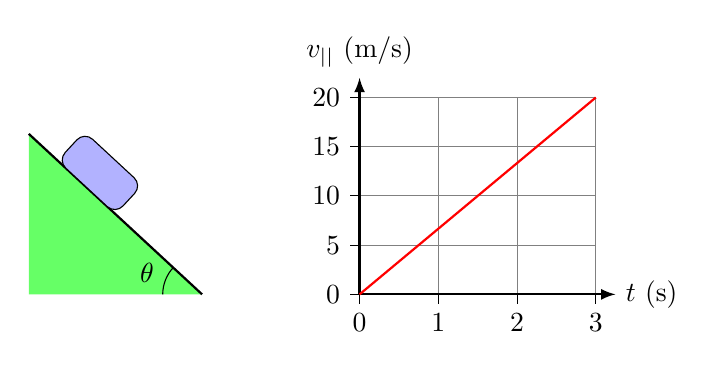
\begin{tikzpicture}[> = latex]

	% Definitions
	
	\def\Q{42.8}
	
	% Ramp + angle indicator
	
	\draw [draw = none, fill = green!60] (0, 0) -- (180 - \Q : 3) -- ({-3 * cos(\Q)}, 0) -- cycle;
	\draw [thick] (0, 0) -- (180 - \Q : 3);
	
	\draw (-0.5, 0) arc (180 : 180 - \Q : 0.5);
	\node at ({180 - 0.5 * \Q} : 0.75) {$\theta$};
	
	% Block
	
	\draw [rotate = -\Q, fill = blue!30, rounded corners] (-2.5, 0) rectangle (-1.5, 0.5);
	
	% Graph axes + labels + grid
	
	\draw [thin, gray, ystep = 0.625 cm] (2, 0) grid (5, 2.51);
	\draw [<->, thick] (2, 2.75) node [above] {$v_{||}$ (m/s)} -- (2, 0) -- (5.25, 0) node [right] {$t$ (s)};
	
	\foreach \x in {0, 1, 2, 3}
		\draw (2 + \x, 0) -- (2 + \x, -0.125) node [below] {$\x$};
		
	\foreach \y in {0, 5, 10, 15, 20}
		\draw (2, 0.125 * \y) -- (1.875, 0.125 * \y) node [left] {$\y$};
		
	% Curve
	
	\draw [thick, red] (2, 0) -- (5, 2.5);

\end{tikzpicture}

\vspace{1em}

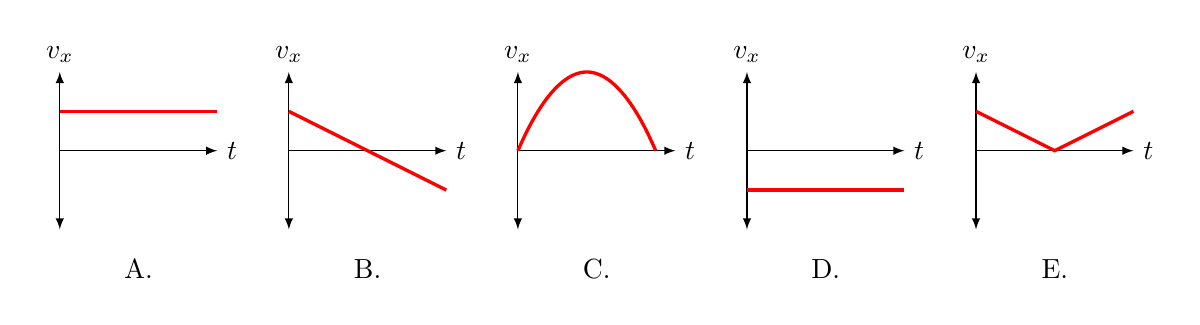
\begin{tikzpicture}[> = latex]
\matrix[column sep = 0.25 cm]{

	% Axes
	
	\draw [<->] (0, -1) -- (0, 1) node [above] {$v_x$};
	\draw [->] (0, 0) -- (2, 0) node [right] {$t$};
	
	% Curve
	
	\draw [very thick, red] (0, 0.5) -- (2, 0.5);
	
	% Label
	
	\node at (1, -1.5) {A.};

&

	% Axes
	
	\draw [<->] (0, -1) -- (0, 1) node [above] {$v_x$};
	\draw [->] (0, 0) -- (2, 0) node [right] {$t$};
	
	% Curve
	
	\draw [very thick, red] (0, 0.5) -- (2, -0.5);
	
	% Label
	
	\node at (1, -1.5) {B.};

&

	% Axes
	
	\draw [<->] (0, -1) -- (0, 1) node [above] {$v_x$};
	\draw [->] (0, 0) -- (2, 0) node [right] {$t$};
	
	% Curve
	
	\draw [very thick, red] (0, 0) parabola bend (0.875, 1) (1.75, 0);
	
	% Label
	
	\node at (1, -1.5) {C.};

&

	% Axes
	
	\draw [<->] (0, -1) -- (0, 1) node [above] {$v_x$};
	\draw [->] (0, 0) -- (2, 0) node [right] {$t$};
	
	% Curve
	
	\draw [very thick, red] (0, -0.5) -- (2, -0.5);
	
	% Label
	
	\node at (1, -1.5) {D.};

&

	% Axes
	
	\draw [<->] (0, -1) -- (0, 1) node [above] {$v_x$};
	\draw [->] (0, 0) -- (2, 0) node [right] {$t$};
	
	% Curve
	
	\draw [very thick, red] (0, 0.5) -- (1, 0) -- (2, 0.5);
	
	% Label
	
	\node at (1, -1.5) {E.};

\\
};

\end{tikzpicture}

\vspace{1em}

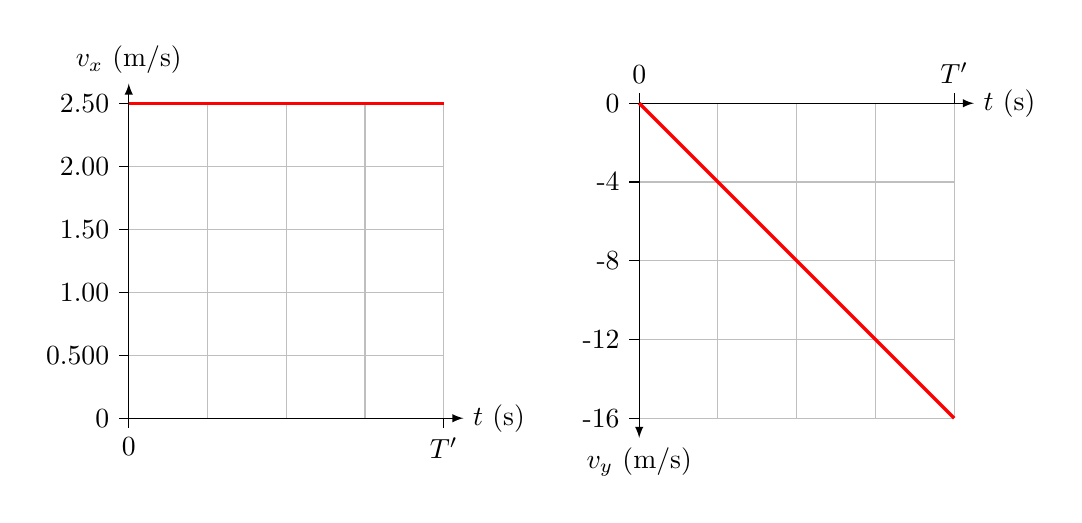
\begin{tikzpicture}[> = latex]
\matrix[column sep = 0.5 cm]{

	% Axes for r_x vs. t graph
	
	\draw [thin, gray!50, ystep = 0.8 cm] (0, 0) grid (4, 4);
	\draw [<->] (0, 4.25) node [above] {$v_x$ (m/s)} -- (0, 0) -- (4.25, 0) node [right] {$t$ (s)};
	
	% Tick marks
	
	\draw (0, 0) -- (0, -0.125) node [below] {0};
	\draw (4, 0) -- (4, -0.125) node [below] {$T'$};
	
	\foreach \y in {0, 0.500, 1.00, 1.50, 2.00, 2.50}
		\draw (0, 1.6 * \y) -- (-0.125, 1.6 * \y) node [left] {\y};
		
	% Curve
	
	\draw [very thick, red] (0, 4) -- (4, 4);

&

	\begin{scope}[yshift = 4 cm]

		% Axes for r_y vs. t graph
		
		\draw [thin, gray!50] (0, 0) grid (4, -4);
		\draw [<->] (0, -4.25) node [below] {$v_y$ (m/s)} -- (0, 0) -- (4.25, 0) node [right] {$t$ (s)};
		
		% Tick marks
		
		\draw (0, 0) -- (0, 0.125) node [above] {0};
		\draw (4, 0) -- (4, 0.125) node [above] {$T'$};
		
		\foreach \y in {0, -4, ..., -16}
			\draw (0, 0.25 * \y) -- (-0.125, 0.25 * \y) node [left] {\y};
			
		% Curve
		
		\draw [very thick, red] (0, 0) -- (4, -4);
	
	\end{scope}

\\	
};

\end{tikzpicture}

\vspace{1em}

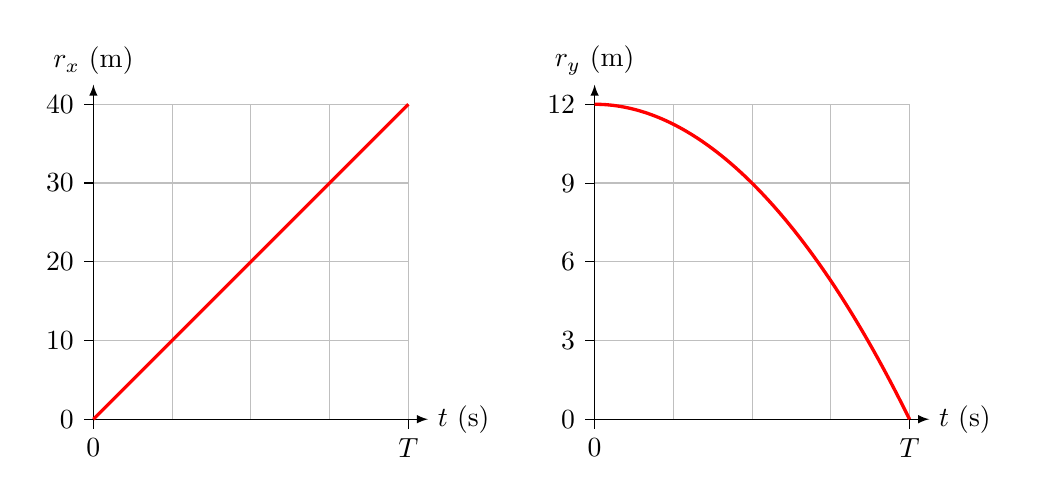
\begin{tikzpicture}[> = latex]
\matrix[column sep = 0.5 cm]{

	% Axes for r_x vs. t graph
	
	\draw [thin, gray!50] (0, 0) grid (4, 4);
	\draw [<->] (0, 4.25) node [above] {$r_x$ (m)} -- (0, 0) -- (4.25, 0) node [right] {$t$ (s)};
	
	% Tick marks
	
	\draw (0, 0) -- (0, -0.125) node [below] {0};
	\draw (4, 0) -- (4, -0.125) node [below] {$T$};
	
	\foreach \y in {0, 10, ..., 40}
		\draw (0, 0.1 * \y) -- (-0.125, 0.1 * \y) node [left] {\y};
		
	% Curve
	
	\draw [very thick, red] (0, 0) -- (4, 4);

&

	% Axes for r_y vs. t graph
	
	\draw [thin, gray!50] (0, 0) grid (4, 4);
	\draw [<->] (0, 4.25) node [above] {$r_y$ (m)} -- (0, 0) -- (4.25, 0) node [right] {$t$ (s)};
	
	% Tick marks
	
	\draw (0, 0) -- (0, -0.125) node [below] {0};
	\draw (4, 0) -- (4, -0.125) node [below] {$T$};
	
	\foreach \y in {0, 3, ..., 12}
		\draw (0, 0.333 * \y) -- (-0.125, 0.333 * \y) node [left] {\y};
		
	% Curve
	
	\draw [very thick, red] (0, 4) parabola (4, 0);

\\	
};

\end{tikzpicture}

\vspace{1em}

\begin{tikzpicture}[> = latex]
	
	% The dot
	
	\filldraw (0, 0) circle (2 pt);
	
	% Coordinate axes
	
	\draw [dashed] (-2, 0) -- (2, 0) node [right] {$+x$};
	\draw [dashed] (0, 2) node [above] {$+y$} -- (0, -2);
	
	% Three forces on ball
	
	\begin{scope}[->, thick]
	
		\draw (0, 0) -- node [above] {$F_N$} (180 : 1.5);
		\draw (0, 0) -- node [right] {$F_g$} (270 : 1.5);
		\draw (0, 0) -- (35 : 1.5) node [above] {$F$};
		
	\end{scope}
	
	% Angle indicator for force F_N
	
	\draw (0.5, 0) arc (0 : 35 : 0.5);
	\node at (17.5 : 0.75) {$\theta$};

\end{tikzpicture}

\vspace{1em}

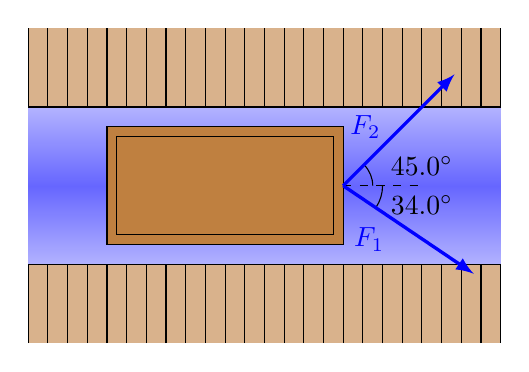
\begin{tikzpicture}[> = latex]

	% The canal water
	
	\draw [top color = blue!30, bottom color = blue!30, middle color = blue!60, draw = none] (-3, -1) rectangle (3, 1);

	% Wooden slats on canal side
	
	\draw [fill = brown!60, draw = none] (-3, 1) rectangle (3, 2);
	\draw [fill = brown!60, draw = none] (-3, -1) rectangle (3, -2);
	
	\foreach \x in {-3, -2.75, ..., 2.75}
	{
		\draw (\x, 2) -- (\x, 1) -- (\x + 0.25, 1) -- (\x + 0.25, 2);
		\draw (\x, -2) -- (\x, -1) -- (\x + 0.25, -1) -- (\x + 0.25, -2);
	}
	
	% Barge
	
	\draw [fill = brown] (-2, -0.75) rectangle (1, 0.75);
	\draw (-1.875, -0.625) rectangle (0.875, 0.625);
	
	% Forces
	
	\draw [dashed] (1, 0) -- (2, 0) node [above] {$45.0^\circ$} node [below] {$34.0^\circ$};
	
	\begin{scope}[thin]
	
		\draw (1.5, 0) arc (0 : -34 : 0.5);
		\draw (1.375, 0) arc (0 : 45 : 0.375);
	
	\end{scope}
	
	\begin{scope}[very thick, blue, ->]
	
		\draw (1, 0) -- node [pos = 0.2, above = 0.5 em] {$F_2$} ++ (45 : 2);
		\draw (1, 0) -- node [pos = 0.2, below = 0.5 em] {$F_1$} ++ (-34 : 2);
	
	\end{scope}

\end{tikzpicture}

\vspace{1em}

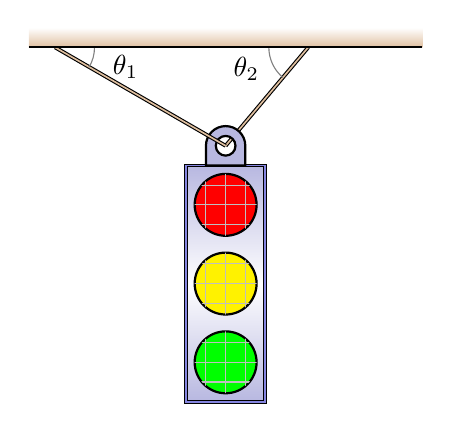
\begin{tikzpicture}

	% Street light
	
	\draw [fill = red, very thick] (0, 1) circle (0.4);
	\draw [fill = yellow, very thick] (0, 0) circle (0.4);
	\draw [fill = green, very thick] (0, -1) circle (0.4);
	
	\draw [thin, gray!50, step = 0.25] (-0.5, -1.5) grid (0.5, 1.5);
	
	\draw [top color = blue!40!gray!40, bottom color = blue!40!gray!40, middle color = white] (-0.5, -1.5) rectangle (0.5, 1.5)
		(0.4, 1) arc (0 : 360 : 0.4)
		(0.4, 0) arc (0 : 360 : 0.4)
		(0.4, -1) arc (0 : 360 : 0.4);
	\draw [double = blue!60!gray!60] (-0.5, -1.5) -- (-0.5, 1.5) -- (0.5, 1.5) -- (0.5, -1.5) -- cycle;
	
	% Connection + cables
	
	\draw [double = brown!50] (0, 1.75) -- ({1.25 / tan(50)}, 3);
	
	\draw [thick, fill = blue!40!gray!40] (-0.25, 1.5) -- (-0.25, 1.75) arc (180 : 0 : 0.25) -- (0.25, 1.5) -- cycle
		(0.125, 1.75) arc (0 : 360 : 0.125);
	
	\draw [double = brown!50] (0, 1.75) -- ({-1.25 / tan(30)}, 3);
	
	% Angle indicators
	
	\draw [thin, gray] ({-1.25 / tan(30) + 0.5}, 3) arc (0 : -30 : 0.5) node [right = 0.5 em, text = black] {$\theta_1$};
	\draw [thin, gray] ({1.25 / tan(50) - 0.5}, 3) node [below left, text = black] {$\theta_2$} arc (180 : 230 : 0.5);
	
	% Ceiling
	
	\draw [bottom color = brown!50, top color = white, draw = none] (-2.5, 3) rectangle (2.5, 3.25);
	\draw [thick] (-2.5, 3) -- (2.5, 3);

\end{tikzpicture}

\vspace{1em}

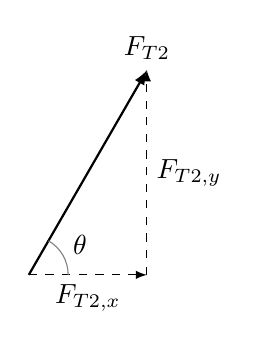
\begin{tikzpicture}[> = latex]
	
	\begin{scope}[->]

		\draw [dashed] (0, 0) -- node [below] {$F_{T2, x}$} ({3 * cos(60)}, 0);
		\draw [dashed] ({3 * cos(60)}, 0) -- node [right] {$F_{T2, y}$} (60 : 3);
		
		\draw [thick] (0, 0) -- (60 : 3) node [above] {$F_{T2}$};
		
	\end{scope}
	
	\draw [gray] (0.5, 0) arc (0 : 60 : 0.5);
	\node at (30 : 0.75) {$\theta$};

\end{tikzpicture}

\vspace{1em}

\begin{tikzpicture}[> = latex]
	
	% The dot
	
	\filldraw (0, 0) circle (2 pt);
	
	% Coordinate axes
	
	\draw [dashed] (-2, 0) -- (2, 0) node [right] {$+x$};
	\draw [dashed] (0, 2) node [above] {$+y$} -- (0, -2);
	
	% Three forces on ball
	
	\begin{scope}[->, thick]
	
		\draw (0, 0) -- node [above] {$F_{T1}$} (180 : 1.5);
		\draw (0, 0) -- node [right] {$F_g$} (270 : 1.5);
		\draw (0, 0) -- (60 : 1.5) node [above] {$F_{T2}$};
		
	\end{scope}
	
	% Angle indicator for force F_T2
	
	\draw (0.5, 0) arc (0 : 60 : 0.5);
	\node at (30 : 0.75) {$\theta$};

\end{tikzpicture}

\vspace{1em}

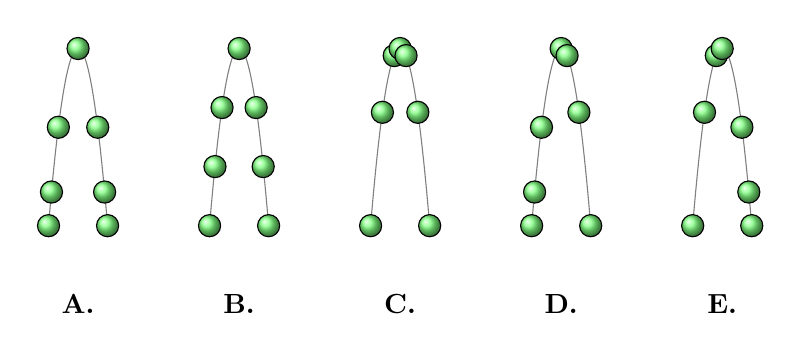
\begin{tikzpicture}
\matrix[column sep = 1 cm]{

	% Parabola
	
	\draw [thin, gray] plot [variable = \x, domain = 0 : 6, samples = 100] ({0.125 * \x}, {-0.25 * (\x - 3)^2 + 2.25});

	% Balls
	
	\foreach \x in {0, 0.3, 1, 3, 5, 5.7, 6}
		\draw [ball color = green!50] (0.125 * \x, {-0.25 * (\x - 3)^2 + 2.25}) circle (4 pt);
		
	% Label
	
	\node at (0.375, -1) {{\bf A.}};
	
&

	% Parabola
	
	\draw [thin, gray] plot [variable = \x, domain = 0 : 6, samples = 100] ({0.125 * \x}, {-0.25 * (\x - 3)^2 + 2.25});

	% Balls
	
	\foreach \x in {0, 0.551, 1.268, 3, 4.732, 5.449, 6}
		\draw [ball color = green!50] (0.125 * \x, {-0.25 * (\x - 3)^2 + 2.25}) circle (4 pt);
		
	% Label
	
	\node at (0.375, -1) {{\bf B.}};
	
&

	% Parabola
	
	\draw [thin, gray] plot [variable = \x, domain = 0 : 6, samples = 100] ({0.125 * \x}, {-0.25 * (\x - 3)^2 + 2.25});

	% Balls
	
	\foreach \x in {0, 1.2, 2.4, 3, 3.6, 4.8, 6}
		\draw [ball color = green!50] (0.125 * \x, {-0.25 * (\x - 3)^2 + 2.25}) circle (4 pt);
		
	% Label
	
	\node at (0.375, -1) {{\bf C.}};
	
&

	% Parabola
	
	\draw [thin, gray] plot [variable = \x, domain = 0 : 6, samples = 100] ({0.125 * \x}, {-0.25 * (\x - 3)^2 + 2.25});

	% Balls
	
	\foreach \x in {0, 0.3, 1, 3, 3.6, 4.8, 6}
		\draw [ball color = green!50] (0.125 * \x, {-0.25 * (\x - 3)^2 + 2.25}) circle (4 pt);
		
	% Label
	
	\node at (0.375, -1) {{\bf D.}};
	
&

	% Parabola
	
	\draw [thin, gray] plot [variable = \x, domain = 0 : 6, samples = 100] ({0.125 * \x}, {-0.25 * (\x - 3)^2 + 2.25});

	% Balls
	
	\foreach \x in {0, 1.2, 2.4, 3, 5, 5.7, 6}
		\draw [ball color = green!50] (0.125 * \x, {-0.25 * (\x - 3)^2 + 2.25}) circle (4 pt);
		
	% Label
	
	\node at (0.375, -1) {{\bf E.}};

\\	
};

\end{tikzpicture}

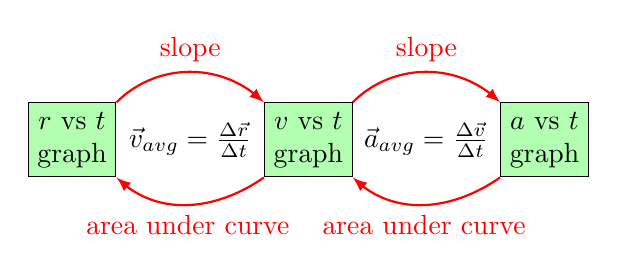
\begin{tikzpicture}[> = latex, graph/.style = {rectangle, draw, fill = green!30, align = center}]

	% Graph type boxes

	\node[graph] (pos) at (0, 0) {$r$ vs $t$\\ graph};
	\node[graph] (vel) at (3, 0) {$v$ vs $t$\\ graph};
	\node[graph] (acc) at (6, 0) {$a$ vs $t$\\ graph};
	
	% Equations
	
	\node at (1.5, 0) {${\vec v}_{avg} = \frac{\Delta {\vec r}}{\Delta t}$};
	\node at (4.5, 0) {${\vec a}_{avg} = \frac{\Delta {\vec v}}{\Delta t}$};
	
	% Arrows for slope, area between graphs
	
	\begin{scope}[->, thick, red]
	
		\draw (pos.north east) to [out = 45, in = 135] node [above] {slope} (vel.north west);
		\draw (vel.south west) to [out = 215, in = 315] node [below] {area under curve} (pos.south east);
	
		\draw (vel.north east) to [out = 45, in = 135] node [above] {slope} (acc.north west);
		\draw (acc.south west) to [out = 215, in = 315] node [below] {area under curve} (vel.south east);
	
	\end{scope}

\end{tikzpicture}

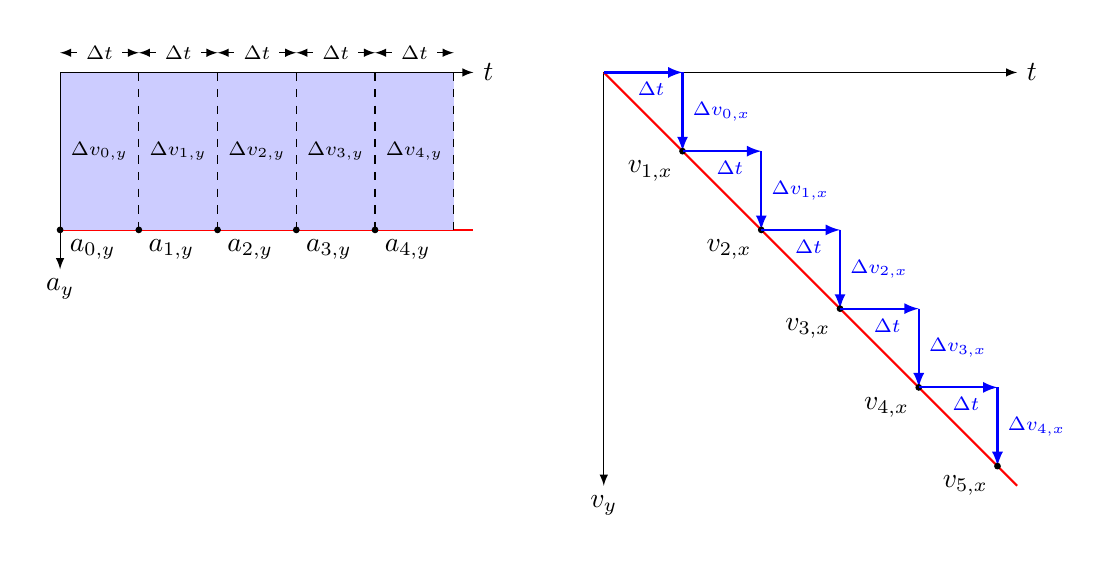
\begin{tikzpicture}[> = latex]
\matrix[column sep = 1 cm]{
	
	% a_x curve
	
	\draw [red, thick] (0, -2) -- (5.25, -2);
	
	% Label sequence of areas under curve
	
	\draw [draw = none, fill = blue!20] (0, 0) rectangle (5, -2);
	
	\foreach \x in {0, 1, ..., 4}
	{
	
		% Define x + 1 as \xn

		\pgfmathtruncatemacro{\xn}{\x + 1}
		
		% Label rectangle areas
		
		\node [font = \scriptsize] at ({\x + 0.5}, -1) {$\Delta v_{\x, y}$};
		\draw [dashed] (\xn, 0) -- (\xn, -2);
		
		% Label dt time steps
		
		\draw [<->] (\x, 0.25) -- node [midway, font = \scriptsize, fill = white] {$\Delta t$} (\xn, 0.25);
		
		% Label a_x used in each update
		
		\draw [fill = black] (\x, -2) circle (1 pt) node [below right] {$a_{\x, y}$};
	}

	% Graph axes
	
	\draw [<->] (0, -2.5) node [below] {$a_y$} -- (0, 0) -- (5.25, 0) node [right] {$t$};

&
	
	% Graph axes
	
	\draw [<->] (0, -5.25) node [below] {$v_y$} -- (0, 0) -- (5.25, 0) node [right] {$t$};

	% r_x curve
	
	\draw [red, thick] (0, 0) -- (5.25, -5.25);
	
	% Label sequence of arrows for updating v_x
	
	\foreach \x in {0, 1, ..., 4}
	{

		% Define x + 1 as \xn

		\pgfmathtruncatemacro{\xn}{\x + 1}
		
		% Label arrows for dt, dv
		
		\draw [blue, thick, ->] (\x, -\x) -- node [pos = 0.6, font = \scriptsize, below] {$\Delta t$} (\xn, -\x);
		\draw [blue, thick, ->] (\xn, -\x) -- node [midway, font = \scriptsize, right] {$\Delta v_{\x, x}$} (\xn, -\xn);
		
		% Create points for updated velocities
		
		\draw [fill = black] (\xn, -\xn) circle (1 pt) node [below left] {$v_{\xn, x}$};
		
	}
	
\\
};
	
\end{tikzpicture}

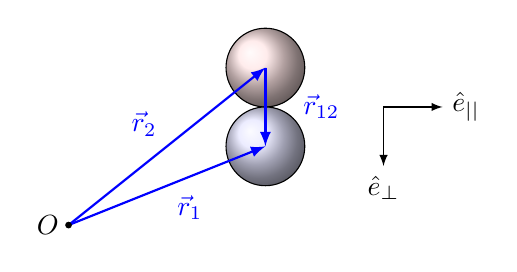
\begin{tikzpicture}[> = latex]

	% Two colliding spheres
	
	\draw [ball color = red!10] (0, 0.5) circle (0.5);
	\draw [ball color = blue!10] (0, -0.5) circle (0.5);
	
	% Position vectors
	
	\begin{scope}[->, thick, blue]
	
		\draw (-2.5, -1.5) -- node [above left] {${\vec r}_2$} (0, 0.5);
		\draw (-2.5, -1.5) -- node [below right] {${\vec r}_1$} (0, -0.5);
		
		\draw (0, 0.5) -- node [right = 1 em] {${\vec r}_{12}$} (0, -0.5);

	\end{scope}
	
	% Parallel, perpendicular unit vectors
	
	\draw [<->] (1.5, -0.75) node [below] {${\hat e}_\perp$} -- (1.5, 0) -- (2.25, 0) node [right] {${\hat e}_{||}$};
	
	% Mark origin
	
	\draw [fill = black] (-2.5, -1.5) circle (1 pt) node [left] {$O$};

\end{tikzpicture}

\vspace{1em}

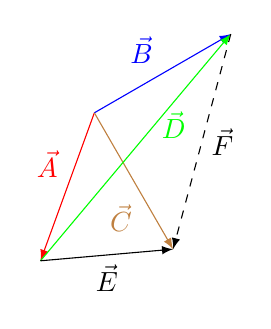
\begin{tikzpicture}[> = latex]

	% A heap of vectors
	
	\begin{scope}[->]
	
		\draw [red] (0, 0) -- node [above left] {${\vec A}$} (250 : 2) coordinate (A-end);
		\draw [blue] (0, 0) -- node [above left] {${\vec B}$} (30 : 2) coordinate (B-end);
		\draw [brown] (0, 0) -- node [pos = 0.60, below left] {${\vec C}$} (300 : 2) coordinate (C-end);
		
		\draw [green] (A-end) -- node [pos = 0.70, below] {${\vec D}$} (B-end);
		\draw (A-end) -- node [below] {${\vec E}$} (300 : 2);
		\draw [dashed] (B-end) -- node [right] {${\vec F}$} (300 : 2);
		
	\end{scope}

\end{tikzpicture}

\vspace{1em}

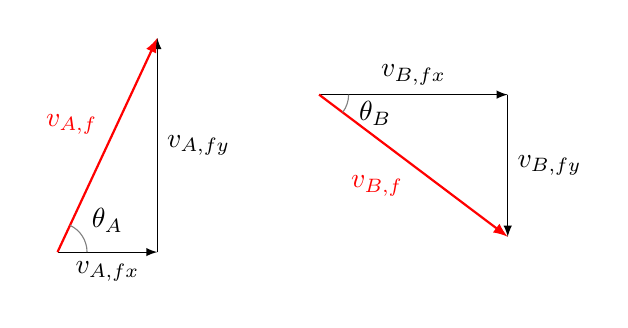
\begin{tikzpicture}[> = latex]
\matrix[column sep = 1 cm]{

	% Vector diagram for v_Af
	
	\draw [->] (0, 0) -- node [below] {$v_{A, fx}$} ({3 * cos(65)}, 0);
	\draw [->] ({3 * cos(65)}, 0) -- node [right] {$v_{A, fy}$} (65 : 3);
	
	\draw [->, thick, red] (0, 0) -- node [above left] {$v_{A, f}$} (65 : 3);
	
	% Angle indicator
	
	\draw [thin, gray] (0.375, 0) arc (0 : 65 : 0.375);
	\node at (32.5 : 0.75) {$\theta_A$};
	
&

	% Vector diagram for v_Bf
	
	\draw [->] (0, 2) -- node [above] {$v_{B, fx}$} ({3 * cos(37)}, 2);
	\draw [->] ({3 * cos(37)}, 2) -- node [right] {$v_{B, fy}$} ({3 * cos(37)}, {2 - 3 * sin(37)});
	
	\draw [->, thick, red] (0, 2) -- node [below left] {$v_{B, f}$} ++ (-37 : 3);
	
	% Angle indicator
	
	\draw [thin, gray] (0.375, 2) arc (0 : -37 : 0.375);
	\node at ({0.75 * cos(18.5)}, {2 - 0.75 * sin(18.5)}) {$\theta_B$};

\\
};

\end{tikzpicture}

\vspace{1em}

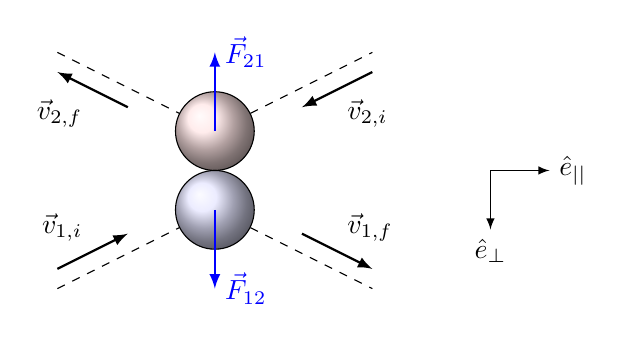
\begin{tikzpicture}[> = latex]

	% Line of motion before, after collision
	
	\begin{scope}[dashed]
	
		\draw (-2, 1.5) -- (0, 0.5) -- (2, 1.5);
		\draw (-2, -1.5) -- (0, -0.5) -- (2, -1.5);
	
	\end{scope}

	% Two colliding spheres
	
	\draw [ball color = red!10] (0, 0.5) circle (0.5);
	\draw [ball color = blue!10] (0, -0.5) circle (0.5);
	
	% Force vectors
	
	\begin{scope}[->, thick, blue]
	
		\draw (0, -0.5) -- (0, -1.5) node [right] {${\vec F}_{12}$};
		\draw (0, 0.5) -- (0, 1.5) node [right] {${\vec F}_{21}$};

	\end{scope}
	
	% Initial, final velocity vectors
	
	\draw [->, thick] (-2, -1.25) -- node [above left] {${\vec v}_{1, i}$} ++ ({atan(0.5)} : 1);
	\draw [<-, thick] (2, -1.25) -- node [above right] {${\vec v}_{1, f}$} ++ ({180 - atan(0.5)} : 1);
	
	\draw [<-, thick] (-2, 1.25) -- node [below left] {${\vec v}_{2, f}$} ++ ({-atan(0.5)} : 1);
	\draw [->, thick] (2, 1.25) -- node [below right] {${\vec v}_{2, i}$} ++ ({180 + atan(0.5)} : 1);
	
	% Parallel, perpendicular unit vectors
	
	\draw [<->] (3.5, -0.75) node [below] {${\hat e}_\perp$} -- (3.5, 0) -- (4.25, 0) node [right] {${\hat e}_{||}$};

\end{tikzpicture}

\vspace{1em}

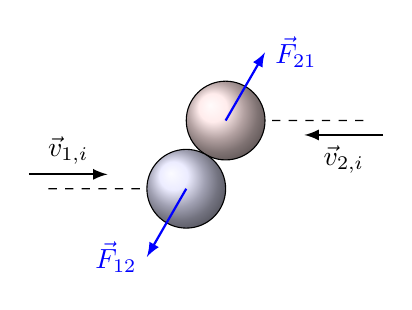
\begin{tikzpicture}

	% Line of motion before collision
	
	\begin{scope}[dashed]
	
		\draw (-2, -0.433) -- (240 : 0.5);
		\draw (2, 0.433) -- (60 : 0.5);
		
	\end{scope}

	% Two colliding spheres
	
	\draw [ball color = red!10] (60 : 0.5) circle (0.5);
	\draw [ball color = blue!10] (240 : 0.5) circle (0.5);
	
	% Incoming velocity vectors, force vectors
	
	\begin{scope}[> = latex, thick, ->]
	
		\draw (-2.25, -0.25) --  node [above] {${\vec v}_{1, i}$} (-1.25, -0.25);
		\draw (2.25, 0.25) -- node [below] {${\vec v}_{2, i}$} (1.25, 0.25);
		
		\draw [blue] (240 : 0.5) -- ++ (240 : 1) node [left] {${\vec F}_{12}$};
		\draw [blue] (60 : 0.5) -- ++ (60 : 1) node [right] {${\vec F}_{21}$};
	
	\end{scope}

\end{tikzpicture}

\vspace{1em}

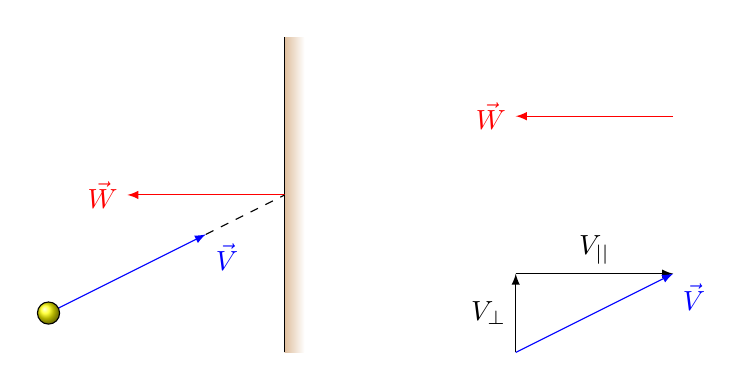
\begin{tikzpicture}[> = latex]
\matrix[column sep = 2 cm]{

	% Wall
	
	\draw [draw = none, left color = brown!50, right color = white] (0, -2) rectangle (0.25, 2);
	\draw (0, -2) -- (0, 2);
	
	% Normal vector
	
	\draw [red, ->] (0, 0) -- (-2, 0) node [left] {${\vec W}$};
	
	% Ball + velocity vector
	
	\draw [blue, ->] (-3, -1.5) -- (-1, -0.5) node [below right] {${\vec V}$};
	\draw [ball color = yellow] (-3, -1.5) circle (4 pt);
	\draw [dashed] (-1, -0.5) -- (0, 0);
	
&

	% Normal vector
	
	\draw [red, ->] (0, 1) -- (-2, 1) node [left] {${\vec W}$};
	
	% Velocity vector + components
	
	\draw [->] (-2, -2) -- node [left] {$V_\perp$} (-2, -1);
	\draw [->] (-2, -1) -- node [above] {$V_{||}$} (0, -1);
	
	\draw [blue, ->] (-2, -2) -- (0, -1) node [below right] {${\vec V}$};

\\
};

\end{tikzpicture}

\vspace{1em}

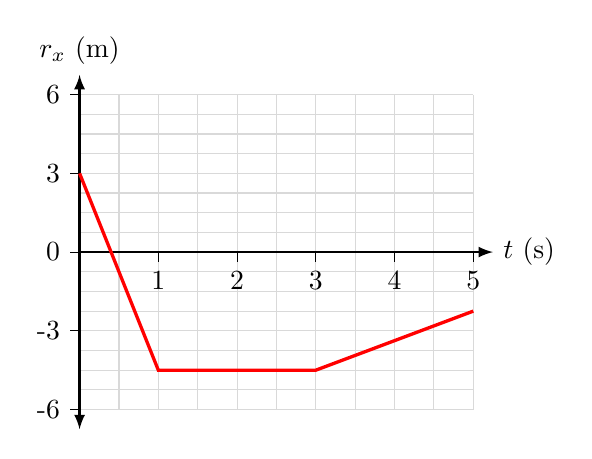
\begin{tikzpicture}[> = latex]

	% Grid
	
	\draw [thin, gray!30, xstep = 0.5 cm, ystep = 0.25 cm] (0, -2) grid (5, 2);

	% Axes
	
	\draw [thick, <->] (0, -2.25) -- (0, 2.25) node [above] {$r_x$ (m)};
	\draw [thick, ->] (0, 0) -- (5.25, 0) node [right] {$t$ (s)};
	
	% Axis labels
	
	\foreach \x in {1, 2, ..., 5}
		\draw (\x, 0) -- (\x, -0.125) node [below] {\x};
	
	\foreach \y in {-6, -3, ..., 6}
		\draw (0, 0.333 * \y) -- (-0.125, 0.333 * \y) node [left] {\y};
		
	% Graph line
	
	\draw [very thick, red] (0, 1) -- (1, -1.5) -- (3, -1.5) -- (5, -0.75);

\end{tikzpicture}

\vspace{1em}

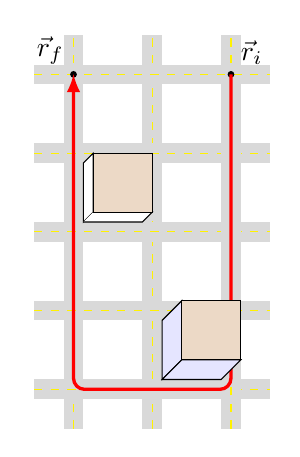
\begin{tikzpicture}
	
	\foreach \x in {-1, 0, 1}
	\foreach \y in {-2, -1, ..., 2}
	{
		% The roads
	
		\draw [fill = gray!30, draw = none] (\x - 0.125, -2.5) rectangle (\x + 0.125, 2.5);
		\draw [fill = gray!30, draw = none] (-1.5, \y - 0.125) rectangle (1.5, \y + 0.125);
		
		% Lane markers in roads
		
		\draw [dashed, yellow] (\x, -2.5) -- (\x, 2.5);
		\draw [dashed, yellow] (-1.5, \y) -- (1.5, \y);
		
	}
	
	% The trip
	
	\draw [fill = black] (1, 2) circle (1 pt) node [above right] {${\vec r}_i$};
	\draw [fill = black] (-1, 2) circle (1 pt) node [above left] {${\vec r}_f$};
	
	\draw [red, very thick, rounded corners, > = latex, ->] (1, 2) -- (1, -2) -- (-1, -2) -- (-1, 2);
	
	% Random buildings
	
	\begin{scope}[yshift = 1 cm]
	
		\draw [fill = white] (-0.875, -0.875) -- (-0.75, -0.75) -- (-0.75, 0) -- (-0.875, -0.125) -- cycle;
		\draw [fill = white] (-0.875, -0.875) -- (-0.125, -0.875) -- (0, -0.75) -- (-0.75, -0.75);
		\draw [fill = brown!30] (-0.75, 0) -- (0, 0) -- (0, -0.75) -- (-0.75, -0.75) -- cycle;
		
	\end{scope}
	
	\draw [fill = blue!10] (0.125, -1.875) -- (0.375, -1.625) -- (0.375, -0.875) -- (0.125, -1.125) -- cycle;
	\draw [fill = blue!10] (0.125, -1.875) -- (0.875, -1.875) -- (1.125, -1.625) -- (0.375, -1.625) -- cycle;
	\draw [fill = brown!30] (0.375, -0.875) -- (1.125, -0.875) -- (1.125, -1.625) -- (0.375, -1.625) -- cycle; 

\end{tikzpicture}

\vspace{1em}

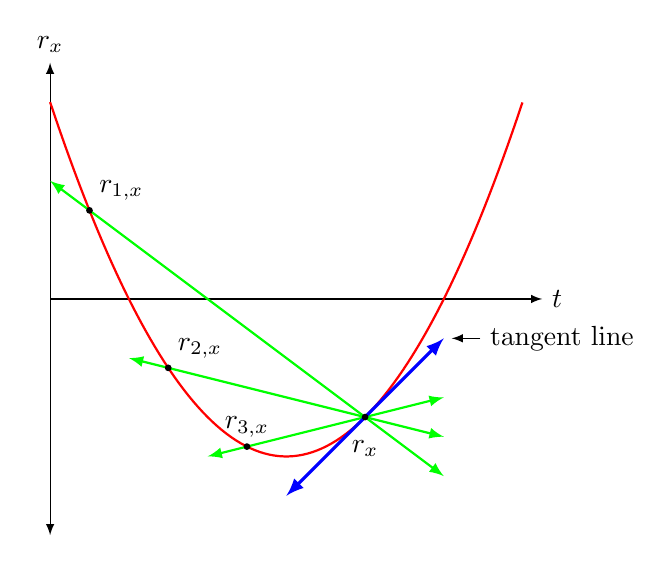
\begin{tikzpicture}[> = latex]

	% Graph axes
	
	\draw [<->] (0, -3) -- (0, 3) node [above] {$r_x$};
	\draw [->] (0, 0) -- (6.25, 0) node [right] {$t$};
	
	% Graph curve
	
	\draw [red, thick] plot [variable = \t, domain = 0 : 6, samples = 100] ({\t}, {0.5 * (\t - 3)^2 - 2});
	
	% Secant line limiting process
	
	\begin{scope}[thick, green, <->]
	
		\draw (0, 1.5) -- (5, -2.25);
		\draw (1, -0.75) -- (5, -1.75);
		\draw (2, -2) -- (5, -1.25);
	
	\end{scope}
	
	\draw [fill = black] (0.5, 1.125) circle (1 pt) node [above right] {$r_{1, x}$};
	\draw [fill = black] (1.5, -0.875) circle (1 pt) node [above right] {$r_{2, x}$};
	\draw [fill = black] (2.5, -1.875) circle (1 pt) node [above] {$r_{3, x}$};
	
	% Tangent line
	
	\draw [very thick, blue, <->] (3, -2.5) -- (5, -0.5);
	\draw [fill = black] (4, -1.5) circle (1 pt) node [below = 0.5 em] {$r_x$};
	
	\node (secant) at (6.5, -0.5) {tangent line};
	\draw [->] (secant.west) -- (5.1, -0.5);
	
\end{tikzpicture}

\vspace{1em}

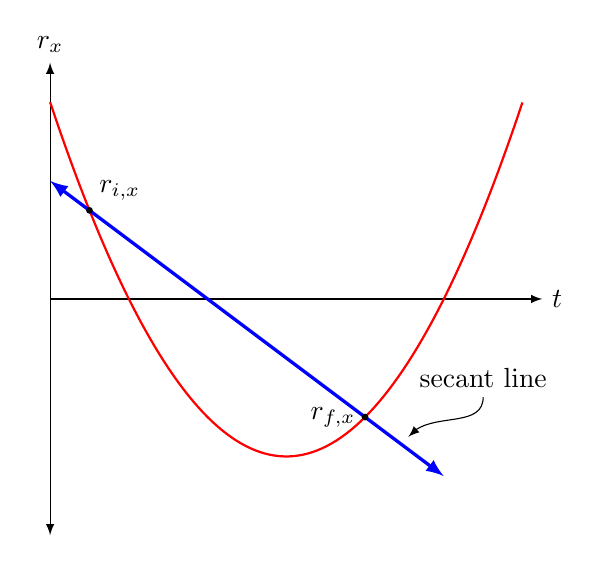
\begin{tikzpicture}[> = latex]

	% Graph axes
	
	\draw [<->] (0, -3) -- (0, 3) node [above] {$r_x$};
	\draw [->] (0, 0) -- (6.25, 0) node [right] {$t$};
	
	% Graph curve
	
	\draw [red, thick] plot [variable = \t, domain = 0 : 6, samples = 100] ({\t}, {0.5 * (\t - 3)^2 - 2});
	
	% Secant line
	
	\draw [very thick, blue, <->] (0, 1.5) -- (5, -2.25);
	\draw [fill = black] (0.5, 1.125) circle (1 pt) node [above right] {$r_{i, x}$};
	\draw [fill = black] (4, -1.5) circle (1 pt) node [left] {$r_{f, x}$};
	
	\node (secant) at (5.5, -1) {secant line};
	\draw [->] (secant.south) to [out = 270, in = 53.1] (4.55, -1.75);
	
\end{tikzpicture}

\vspace{1em}

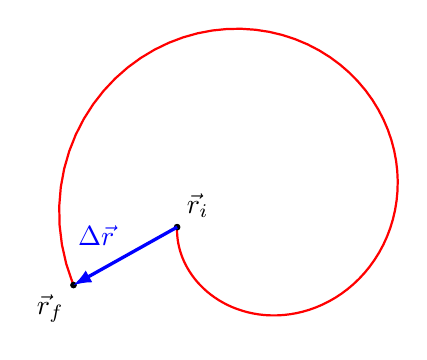
\begin{tikzpicture}

	% Spiral
	
	\draw [red, thick] plot [variable = \t, domain = 1 : 2.5, samples = 100] ({100 * 2^\t} : \t);
	
	% Initial, final points + displacement
	
	\draw [fill = black] (200 : 1) circle (1 pt) node [above right] {${\vec r}_i$};
	\draw [fill = black] (100 * 2^2.5 : 2.5) circle (1 pt) node [below left] {${\vec r}_f$};
	
	\draw [> = latex, ->, very thick, blue] (200 : 1) -- node [above left] {$\Delta {\vec r}$} (100 * 2^2.5 : 2.5);
	
\end{tikzpicture}

\vspace{1em}

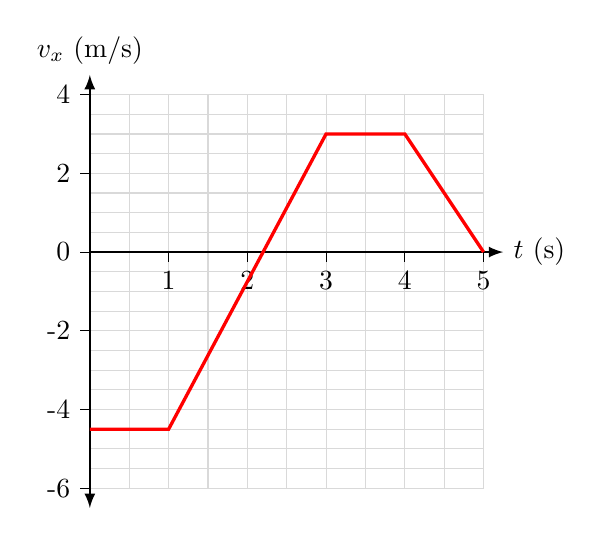
\begin{tikzpicture}[> = latex]

	% Grid
	
	\draw [thin, gray!30, xstep = 0.5 cm, ystep = 0.25 cm] (0, -3) grid (5, 2);

	% Axes
	
	\draw [thick, <->] (0, -3.25) -- (0, 2.25) node [above] {$v_x$ (m/s)};
	\draw [thick, ->] (0, 0) -- (5.25, 0) node [right] {$t$ (s)};
	
	% Axis labels
	
	\foreach \x in {1, 2, ..., 5}
		\draw (\x, 0) -- (\x, -0.125) node [below] {\x};
	
	\foreach \y in {-6, -4, ..., 4}
		\draw (0, 0.5 * \y) -- (-0.125, 0.5 * \y) node [left] {\y};
		
	% Graph line
	
	\draw [very thick, red] (0, -2.25) -- (1, -2.25) -- (3, 1.5) -- (4, 1.5) -- (5, 0);

\end{tikzpicture}

\vspace{1em}

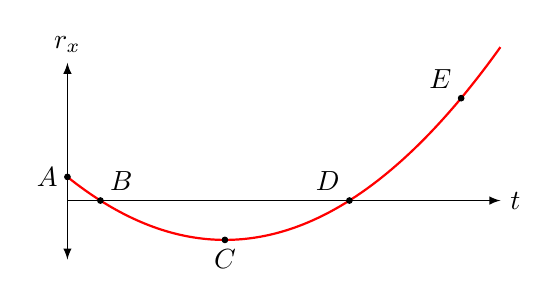
\begin{tikzpicture}[> = latex]

	% Graph axes
	
	\draw [<->] (0, 1.75) node [above] {$r_x$} -- (0, -0.75);
	\draw [->] (0, 0) -- (5.5, 0) node [right] {$t$};
	
	% Graph curve
	
	\draw [red, thick] plot [variable = \t, domain = 0 : 5.5, samples = 100] ({\t}, {0.2 * (\t - 2)^2 - 0.5});
	
	% Marked points
	
	\draw [fill = black] (0, 0.3) circle (1 pt) node [left] {$A$};
	\draw [fill = black] (0.4189, 0) circle (1 pt) node [above right] {$B$};
	\draw [fill = black] (2, -0.5) circle (1 pt) node [below] {$C$};
	\draw [fill = black] (3.581, 0) circle (1 pt) node [above left] {$D$};
	\draw [fill = black] (5, 1.3) circle (1 pt) node [above left] {$E$};
	
\end{tikzpicture}

\vspace{1em}

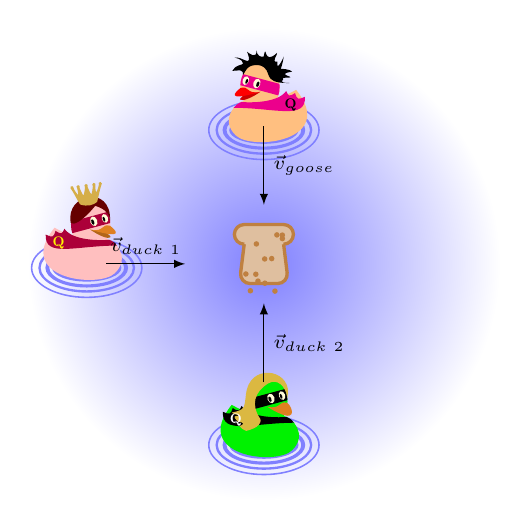
\begin{tikzpicture}[> = latex]

	% Definition
	
	\def\L{0.5}	% Scale for piece of bread

	% Pond
	
	\draw [inner color = blue!50, outer color = white, draw = none] (0, 0) circle (3 cm);
	
	% Quackaluso
	
	\duck [body = orange!50, bill = red, mask = magenta, laughing, cape= magenta, crazyhair = black, water=blue!50,  xshift = -0.5 cm, yshift = 1.5 cm, scale = 0.5] {duck};
	\node[xshift=-2, yshift=-5.5, scale = 0.5] at (tail) {$\textbf{\textcolor{black}Q}$};
	
	\draw [->] (0, 1.75) -- node [right, font = \scriptsize] {${\vec v}_{goose}$} ++ (0, -1);
	
	% Quackier
	
	\duck [body = pink, parting = red!40!black, laughing, queencrown = yellow!30!brown ,  mask = purple!90!black, cape = purple!90!black, water=blue!50,  scale = 0.5, xshift = -3.5 cm, yshift = -0.5 cm, xscale = -1] {duck};

	\node[xshift=1.5, yshift=-5.5, scale = 0.5] at (tail) {$\textbf{\textcolor{yellow}Q}$};
	
	\draw [->] (-2, 0) -- node [above, font = \scriptsize] {${\vec v}_{duck \ 1}$} ++ (1, 0);

	% Quackeene
	
	\duck [body = green!95!black, longhair = yellow!40!brown, mask = black, cape = black, water=blue!50, scale = 0.5, xshift = 1 cm, yshift =-5 cm, xscale = -1] {duck};
	\node[xshift=1.5, yshift=-5.5, scale = 0.5] at (tail) {$\textbf{\textcolor{white}Q}$};
	
	\draw [->] (0, -1.5) -- node [right, font = \scriptsize] {${\vec v}_{duck \ 2}$} ++ (0, 1);
	
	% Bread
	
	\draw [very thick, brown, fill = brown!50] (0.5 * \L, 0.5 * \L) arc (-90 : 90 : 0.25 * \L) -- (-0.5 * \L, \L) arc (90 : 270 : 0.25 * \L) [rounded corners] (-0.5 * \L, 0.5 * \L) -- (-0.625 * \L, -0.5 * \L) -- (0.625 * \L, -0.5 * \L) -- (0.5 * \L, 0.5 * \L);
	
	\foreach \n in {1, ..., 12}{
		\draw [draw = none, fill = brown] (0.5 * \L * rand, 0.75 * \L * rand) circle (1 pt);
	}

\end{tikzpicture}

\begin{tikzpicture}[> = latex, every node/.style = {text = black}]

	% Definitions
	
	\def\Q{12}		% Vector angle
	\def\M{2}		% Magnitude of vector
	\def\R{1}		% Radius of angle indicator angle

	% Cardinal directions
	
	\begin{scope}[<->]
	
		\draw (-3, 0) -- (3, 0) node [above] {$+x$};
		\draw (0,-1.5) -- (0, 1.5) node [left] {$+y$};
	
	\end{scope}
	
	% Actual vector with angle indicator
	
	\draw [thick, red, ->] (0, 0) -- (-\Q : \M);
	\draw [thin, gray] (\R, 0) arc (0 : -\Q : \R);
	\node [font = \scriptsize] at ({-0.5 * \Q} : {1.5 * \R})  {\Q$^\circ$};

\end{tikzpicture}

\begin{tikzpicture}[> = latex]

	% Axes
	
	\draw [<->] (-2, 0) -- (2, 0) node [right] {$+x$};
	\draw [<->] (0, -2) -- (0, 2) node [above] {$+y$};
	
	% Vector
	
	\draw [red, thick, ->] (0, 0) -- (240 : 2) node [left] {${\vec A}$};
	
	% Angle indicator
	
	\draw [gray!50, thin, ->] (1, 0) arc (0 : 240 : 1);
	\node [above left] at (120 : 1) {$240^\circ$};
	
	% Vector diagram
	
	\draw [red, thick, ->] (5, 1) -- node [near end, above left] {${\vec A}$} ++ (240 : 2);
	\draw [dashed] (5, 1) -- node [right] {$A_y$} (5, {1 + 2 * sin(240)}) -- node [below] {$A_x$} (4, {1 + 2 * sin(240)});
	
	\draw [gray!50] (4.75, {1 + 2 * sin(240)}) -- (4.75, {1.25 + 2 * sin(240)}) -- (5, {1.25 + 2 * sin(240)});
	\draw [gray!50] (5, 0.5) node [below left, font = \scriptsize, color = black] {$\theta$} arc (270 : 240 : 0.5);

\end{tikzpicture}

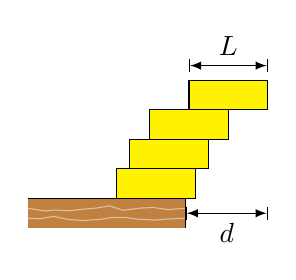
\begin{tikzpicture}[> = latex]

	\pgfmathsetseed{4321}	% Set randomization seed here, so wood grain does not change when overlay slide does

	% Definitions
	
	\def\H{1.2}			% Height of table
	\def\t{0.375}		% Table, leg thickness

	% Table surface, with wood grain
			
	\filldraw [brown, draw = none] (-2, 0) rectangle (0, \t);
	\foreach \m in {1, 2}
		\draw [brown!50, decorate, decoration = {random steps, segment length = 5 pt, amplitude = 1 pt}]
			(-2, \t * \m / 3) -- (0, \t * \m / 3);
	\draw (-2, \t) -- (0, \t) -- (0, 0);
			
	% Blocks
	
	\foreach \N/\d in {1/-0.375, 2/-0.2083, 3/0.04167, 4/0.5417}
		\draw [fill = yellow] ({-0.5 + \d}, \N * \t) rectangle ({0.5 + \d}, {(\N + 1) * \t});
		
	% Distance labels
	
	\draw [|<->|] (0, 0.5 * \t) -- node [below] {$d$} (1.042, 0.5 * \t);
	\draw [|<->|] (0.04167, 5.5 * \t) -- node [above] {$L$} (1.042, 5.5 * \t);

\end{tikzpicture}

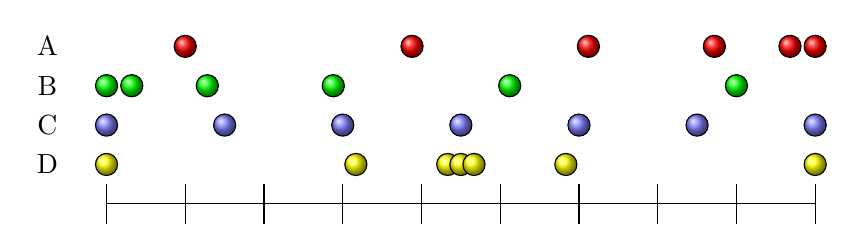
\begin{tikzpicture}

	% Distance ruler
	
	\draw (0, 0) -- (9, 0);
	
	\foreach \n in {0, 1, ..., 9}
		\draw (\n, 0.25) -- (\n, -0.25);
		
	% Ball with constant leftward acceleration
	
	\foreach \x in {1, 2, ..., 6}
		\draw [ball color = red] (-0.32 * \x * \x + 3.84 * \x - 2.52, 2) circle (4 pt);
		
	% Ball with constant rightward acceleration
	
	\foreach \x in {1, 2, ..., 6}
		\draw [ball color = green] (0.32 * \x * \x - 3.84 * \x + 11.52, 1.5) circle (4 pt);
		
	% Ball with constant velocity
	
	\foreach \x in {0, 1, ..., 6}
		\draw [ball color = blue!50] (1.5 * \x, 1) circle (4 pt);
		
	% Ball slowing down, then speeding up
	
	\foreach \x in {0, 1, ..., 6}
		\draw [ball color = yellow] (0.5 * \x * \x * \x / 3 - 1.5 * \x * \x + 4.5 * \x, 0.5) circle (4 pt);
		
	% Labels
	
	\foreach \y/\s in {2/A, 1.5/B, 1/C, 0.5/D}
		\node at (-0.75, \y) {\s};

\end{tikzpicture}

\vspace{1em}

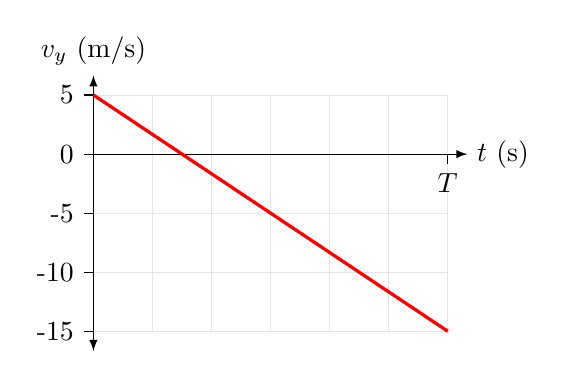
\begin{tikzpicture}[> = latex]

	% Axes + grid
	
	\draw [very thin, gray!20, step = 0.75 cm] (0, 0) grid (4.5, 3);
	
	\draw [<->] (0, -0.25) -- (0, 3.25) node [above] {$v_y$ (m/s)};
	\draw [->] (0, 2.25) -- (4.75, 2.25) node [right] {$t$ (s)};

	% Axis labels
	
	\draw (4.5, 2.25) -- (4.5, 2.125) node [below] {$T$};
	
	\foreach \y in {5, 0, ..., -15}
		\draw (0, {0.15 * \y + 2.25}) -- (-0.125, {0.15 * \y + 2.25}) node [left] {\y};
		
	% Curve
	
	\draw [very thick, red] (0, 3) -- (4.5, 0);

\end{tikzpicture}

\begin{tikzpicture}[> = latex]

\matrix[column sep = 0.5 cm]{

	% Initial momentum
	
	\draw [thick, ->] (0, 0) -- node [midway, above right] {${\vec p}_i$} (150 : 1.5);
	
&

	% Final momentum
	
	\draw [thick, ->] (0, 0.75) -- node [midway, above left] {${\vec p}_f$} ++ (210 : 1.5);
	
&

	% Possible impulse
	
	\draw [thick, red, ->] (0, -0.375) -- (0, 1.125);
	
	% Choice label
	
	\node at (0, -1) {$A.$};
	
&

	% Possible impulse
	
	\draw [thick, red, ->] (0, 1.125) -- (0, -0.375);
	
	% Choice label
	
	\node at (0, -1) {$B.$};
	
&

	% Possible impulse
	
	\draw [thick, red, ->] (0, 0.375) -- (1.5, 0.375);
	
	% Choice label
	
	\node at (0.75, -1) {$C.$};
	
&

	% Possible impulse
	
	\draw [thick, red, ->] (1.5, 0.375) -- (0, 0.375);
	
	% Choice label
	
	\node at (0.75, -1) {$D.$};

\\
};

\end{tikzpicture}

\begin{tikzpicture}

\matrix[row sep = 1 em]{

	% Grid
	
	\draw [thin, gray!20, step = 0.25 cm] (-0.5, -0.5) grid (6.5, 0.5);
		
	% Motion of ball
	
	\foreach \x in {0, 1, 2, 3}
		\draw [ball color = yellow] (2 * \x, 0) circle (4 pt); 
	
	% Label motion
	
	\node at (-1, 0) {$A.$};

\\

	% Grid
	
	\draw [thin, gray!20, step = 0.25 cm] (-0.5, -0.5) grid (6.5, 0.5);
		
	% Motion of ball
	
	\foreach \x in {0, 1, ..., 6}
		\draw [ball color = yellow] (\x, 0) circle (8 pt);
	
	% Label motion
	
	\node at (-1, 0) {$B.$};

\\

	% Grid
	
	\draw [thin, gray!20, step = 0.25 cm] (-0.5, -0.5) grid (6.5, 1.25);
		
	% Motion of ball
	
	\foreach \x in {0, 1, 2, 3}
		\draw [ball color = yellow] (2 * \x, 0.25 * \x) circle (4 pt);
	
	% Label motion
	
	\node at (-1, 0.375) {$C.$};

\\

	% Grid
	
	\draw [thin, gray!20, step = 0.25 cm] (-0.5, -0.5) grid (6.5, 0.5);
		
	% Motion of ball
	
	\foreach \x in {0, 1, ..., 6}
		\draw [ball color = yellow] (\x, 0) circle (4 pt);
	
	% Label motion
	
	\node at (-1, 0) {$D.$};

\\

	% Grid
	
	\draw [thin, gray!20, step = 0.25 cm] (-0.5, -0.5) grid (6.5, 0.5);
		
	% Motion of ball
	
	\foreach \x in {0, 1, 2, 3}
		\draw [ball color = yellow] (2 * \x, 0) circle (8 pt);
	
	% Label motion
	
	\node at (-1, 0) {$E.$};

\\
};

\end{tikzpicture}

\vspace{1em}

\begin{tikzpicture}

\matrix[row sep = 1 em]{

	% Grid
	
	\draw [thin, gray!20, step = 0.25 cm] (-5, -0.75) grid (5, 0.5);
		
	% Motion of ball
	
	\foreach \x in {0, 1, 2, 3}
		\draw [ball color = blue!50] (-1.5 * \x, 0) circle (4 pt);
		
	\foreach \x in {1, 2, 3, 4}
		\draw [ball color = blue!50] (\x, 0) circle (4 pt);
	
	% Marked location
	
	\node at (0, -0.5) {$P$};
	
	% Label motion
	
	\node at (-5.5, -0.125) {$A.$};

\\

	% Grid
	
	\draw [thin, gray!20, step = 0.25 cm] (-5, -0.75) grid (5, 0.5);
		
	% Motion of ball
	
	\foreach \x in {0, 1, 2, 3}
		\draw [ball color = blue!50] (-1.5 * \x, 0) circle (4 pt);
		
	\foreach \x in {1, 2, 3}
		\draw [ball color = blue!50] (1.5 * \x, 0) circle (4 pt);
	
	% Marked location
	
	\node at (0, -0.5) {$P$};
	
	% Label motion
	
	\node at (-5.5, -0.125) {$B.$};

\\

	% Grid
	
	\draw [thin, gray!20, step = 0.25 cm] (-5, -1) grid (5, 0.5);
		
	% Motion of ball
	
	\foreach \x in {0, 1, 2, 3}
		\draw [ball color = blue!50] (-1.5 * \x, 0) circle (4 pt);
		
	\foreach \x in {1, 2, 3}
		\draw [ball color = blue!50] (1.5 * \x, -0.25 * \x) circle (4 pt);
	
	% Marked location
	
	\node at (0, -0.5) {$P$};
	
	% Label motion
	
	\node at (-5.5, -0.25) {$C.$};

\\

	% Grid
	
	\draw [thin, gray!20, step = 0.25 cm] (-5, -0.75) grid (5, 0.5);
		
	% Motion of ball
	
	\foreach \x in {0, 1, 2, 3}
		\draw [ball color = blue!50] (-1.5 * \x, 0) circle (4 pt);
		
	% The ball stops
	
	\node at (2.5, 0) {The ball stops at point $P$};
	
	% Marked location
	
	\node at (0, -0.5) {$P$};
	
	% Label motion
	
	\node at (-5.5, -0.125) {$D.$};
	
\\
};

\end{tikzpicture}

\vspace{1em}

\begin{tikzpicture}[> = latex]

	% Definitions
	
	\def\R{6}		% Scale for range; equal to v_i ^2 / g

	% Floor surface
	
	\filldraw [top color = green!50, bottom color = white, draw = white] ({-0.5 * \R - 0.5}, 0) rectangle ({0.5 * \R + 0.5}, -0.25);
	\draw [thick] ({-0.5 * \R - 0.5}, 0) -- ({0.5 * \R + 0.5}, 0);
	
	% Trajectory
	
	\draw ({-0.5 * \R}, 0) plot [variable = \x, domain = 0 : \R] ({\x - 0.5 * \R}, {\x * tan(45) - \x^2 / (2 * \R * (cos(45))^2)});
	
	% Marked points w/ velocity vector
	
	\coordinate (left) at (-0.375 * \R, {0.125 * \R * tan(45) - 0.015625 * \R / (2 * (cos(45))^2)});
	\draw [blue, thick, ->] (left) -- ++ (1, 0) node [right] {$v_x$};
	\draw [blue, thick, ->] (left) -- ++ (0, 0.75) node [above] {$v_y$};
	\draw [red, thick, ->] (left) -- ++ (1, 0.75) node [above] {${\vec v}$};
	\draw [fill = black] (left) circle (1 pt);
	
	\coordinate (top) at (0, {0.5 * \R * tan(45) - 0.25 * \R / (2 * (cos(45))^2)});
	\draw [red, thick, ->] (top) -- node [above] {${\vec v} = v_x {\hat x}$} ++ (1, 0);
	\draw [fill = black] (top) circle (1 pt);
	
	\coordinate (right) at (0.375 * \R, {0.875 * \R * tan(45) - 0.765625 * \R / (2 * (cos(45))^2)});
	\draw [blue, thick, ->] (right) -- ++ (1, 0) node [right] {$v_x$};
	\draw [blue, thick, ->] (right) -- ++ (0, -0.75) node [above left] {$v_y$};
	\draw [red, thick, ->] (right) -- ++ (1, -0.75) node [below] {${\vec v}$};
	\draw [fill = black] (right) circle (1 pt);

\end{tikzpicture}

\begin{tikzpicture}[font = \footnotesize]

	% Definitions
	
	\def\R{5}		% Scale for range; equal to v_i ^2 / g

	% Floor surface
	
	\filldraw [top color = green!50, bottom color = white, draw = white] (-3, 0) rectangle (3, -0.25);
	\draw [thick] (-3, 0) -- (3, 0);
	
	% Trajectories
	
	\draw [thick] (-2.5, 0) plot [variable = \x, domain = 0 : 4.33] ({\x - 2.5}, {\x * tan(30) - \x^2 / (2 * \R * (cos(30))^2)});
	\node [below] at (-0.3349, 0.6250) {$\theta = 30.0^\circ$};
	
	\draw [thick] (-2.5, 0) plot [variable = \x, domain = 0 : 4.33] ({\x - 2.5}, {\x * tan(60) - \x^2 / (2 * \R * (cos(60))^2)});
	\node [above] at (-0.3349, 1.875) {$\theta = 60.0^\circ$};
	
	\draw [blue, thick] (-2.5, 0) plot [variable = \x, domain = 0 : 5] ({\x - 2.5}, {\x * tan(45) - \x^2 / (2 * \R * (cos(45))^2)}) node [above right] {$\theta = 45.0^\circ$};

\end{tikzpicture}

\begin{tikzpicture}[> = latex]

	\draw [thick, blue, ->] (0, 0) -- node [midway, below left] {$v_f$} (-49 : 3.8);
	\draw [->] (0, 0) -- node [midway, above] {$v_{f, x}$} ({3.8 * cos(49)}, 0);
	\draw [->] ({3.8 * cos(49)}, 0) -- node [midway, right] {$v_{f, y}$} (-49 : 3.8);
	\node at (-25 : 0.75) {$\theta_f$};

\end{tikzpicture}

\vspace{1em}

\begin{tikzpicture}[> = latex]

	\draw [thick, blue, ->] (0, 0) -- node [midway, above left] {$v_i$} (35 : 3);
	\draw [->] (0, 0) -- node [midway, below] {$v_{i, x}$} ({3 * cos(35)}, 0);
	\draw [->] ({3 * cos(35)}, 0) -- node [midway, right] {$v_{i, y}$} (35 : 3);
	\node at (17.5 : 0.75) {$\theta_i$};

\end{tikzpicture}

\begin{tikzpicture}[> = latex]

	% Displacements
	
	\draw [draw = none, fill = blue!20] (1, 0) -- (1, 0.5417) plot [variable = \t, domain = 1 : 2] ({\t}, {\t^3 / 6 - 1.25 * \t^2 + 3.125 * \t - 1.5}) -- (2, 0) -- (1, 0);
	\draw [draw = none, fill = blue!20] (3, 0) -- (3, 1.125) plot [variable = \t, domain = 3 : 4] ({\t}, {\t^3 / 6 - 1.25 * \t^2 + 3.125 * \t - 1.5}) -- (4, 0) -- (3, 0);

	% v_x curve
	
	\draw [red, thick] plot [variable = \t, domain = 0 : 4.5] ({\t}, {\t^3 / 6 - 1.25 * \t^2 + 3.125 * \t - 1.5});
	
	% Various marked points
	
	\draw [fill = black] (1, 0.5417) circle (1 pt) node [above left] {$v_{1, x}$};
	\draw [dashed] (1, 0) -- (1, 0.5417);
	
	\draw [fill = black] (2, 1.083) circle (1 pt) node [above left] {$v_{2, x}$};
	\draw [dashed] (2, 0) -- (2, 1.083);
	
	\draw [|<->|] (1, -0.25) -- node [midway, below] {$t_1$} (2, -0.25);
	
	\draw [fill = black] (3, 1.125) circle (1 pt) node [above] {$v_{3, x}$};
	\draw [dashed] (3, 0) -- (3, 1.125);
	
	\draw [fill = black] (4, 1.667) circle (1 pt) node [below right] {$v_{4, x}$};
	\draw [dashed] (4, 0) -- (4, 1.667);
	
	\draw [|<->|] (3, -0.25) -- node [midway, below] {$t_2$} (4, -0.25);
	
	% Graph axes
	
	\draw [<->] (0, 2.5) node [above] {$v_x$} -- (0, -1.75);
	\draw [->] (0, 0) -- (4.75, 0) node [right] {$t$};

\end{tikzpicture}

\begin{tikzpicture}[> = latex]
	
	% v_x curve
	
	\draw [red, thick] (0, 0) parabola bend (2.5, 2) (5, 0);
	
	% Various marked points
	
	\draw [fill = black] (1, 32/25) circle (1 pt) node [above left] {$v_{1, x}$};
	\draw [dashed] (1, 0) -- (1, 32/25);
	
	\draw [fill = black] (2, 48/25) circle (1 pt) node [above left] {$v_{2, x}$};
	\draw [dashed] (2, 0) -- (2, 48/25);
	
	\draw [|<->|] (1, -0.25) -- node [midway, below] {$t_1$} (2, -0.25);
	
	\draw [fill = black] (3, 48/25) circle (1 pt) node [above right] {$v_{3, x}$};
	\draw [dashed] (3, 0) -- (3, 48/25);
	
	\draw [fill = black] (4, 32/25) circle (1 pt) node [above right] {$v_{4, x}$};
	\draw [dashed] (4, 0) -- (4, 32/25);
	
	\draw [|<->|] (3, -0.25) -- node [midway, below] {$t_2$} (4, -0.25);
	
	% Graph axes
	
	\draw [<->] (0, 2.75) node [above] {$v_x$} -- (0, 0) -- (5.25, 0) node [right] {$t$};

\end{tikzpicture}

\begin{tikzpicture}[> = latex]
	
	% Displacement
	
	\draw [draw = none, fill = blue!20] (2, 0) -- (2, -1.2) -- (4, -2.4) -- (4, 0) -- (2, 0);
	\draw [dashed] (2, 0) -- (2, -1.2);
	\draw [dashed] (4, 0) -- (4, -2.4);
	
	\node at (3, -0.9) {$\Delta r_x$};
	\draw [|<->|] (2, 0.25) -- node [midway, above] {$t$} (4, 0.25);
	
	% Graph axes
	
	\draw [<->] (0, -3.25) node [below] {$v_x$} -- (0, 0) -- (5.25, 0);

	% v_x curve
	
	\draw [red, thick] (0, 0) -- (5, -3);
	
	% Initial, final velocities
	
	\draw [fill = black] (2, -1.2) circle (1 pt) node [below left] {$v_{i, x}$};
	\draw [fill = black] (4, -2.4) circle (1 pt) node [below left] {$v_{f, x}$};

\end{tikzpicture}

\begin{tikzpicture}

	% Definitions
	
	\def\X{5}		% x, y sizes of grid
	\def\Y{2.5}
	
	\def\Xmax{10}	% Maximum values along each axis
	\def\Ymax{6}

	% Axes with tick marks, labels
	
	\foreach \N in {2, 4, ..., \Xmax}
	{
		\draw [gray!30] ({\X * \N / \Xmax}, 0) -- ({\X * \N / \Xmax}, \Y);
		\node at ({\X * \N / \Xmax}, 0) [below] {\N};
	}
	
	\foreach \M in {0, 3, ..., \Ymax}
	{
		\draw [gray!30] (0, {\Y * \M / \Ymax}) -- (\X, {\Y * \M / \Ymax});
		\node at (0, {\Y * \M / \Ymax}) [left] {\M};
	}
	
	\draw [thick, > = latex, <->] (1.1 * \X, 0) -- (0, 0) -- (0, 1.2 * \Y);
	
	\node at ({\X / 2}, 0) [below = 1 em] {$t$ (s)};
	\node at (0, {3 * \Y / \Ymax}) [rotate = 90, above = 1 em] {$a_x$ (m/s$^2$)};
	
	% Graph line
	
	\draw [very thick, red] (0, 0) -- ({2 * \X / \Xmax}, 0)
		-- ({2 * \X / \Xmax}, {6 * \Y / \Ymax}) -- ({8 * \X / \Xmax}, {6 * \Y / \Ymax})
		-- ({8 * \X / \Xmax}, {3 * \Y / \Ymax}) -- ({10 * \X / \Xmax}, {3 * \Y / \Ymax})
		-- ({10 * \X / \Xmax}, 0) -- (\X, 0);

\end{tikzpicture}

\begin{tikzpicture}[> = latex]

	% Distance ruler
	
	\draw (0, 0) -- (8, 0);
	
	\foreach \n in {0, 1, ..., 8}
		\draw (\n, 0.25) -- (\n, -0.25);
		
	% Ball with constant acceleration
	
	\foreach \x in {1, 2, ..., 6}
	{
		\draw [ball color = gray] (-0.32 * \x * \x + 3.84 * \x - 3.52, -0.5) circle (4 pt);
		\draw [ball color = green] (0.32 * \x * \x - 0.64 * \x + 0.32, 0.5) circle (4 pt);
	}
	
	% Average velocity vectors
	
	\foreach \x in {1, 2, 3, 4}
	{
		\draw [gray, thick , ->] (-0.32 * \x * \x + 8, -0.75) -- node [below, midway] {${\vec v}_{\x, avg}$} (-0.32 * \x * \x -0.64 * \x + 7.68, -0.75);
		\draw [green, thick , ->] (0.32 * \x * \x - 3.84 * \x + 11.52, 0.75) -- node [above, midway] {${\vec v}_{\x, avg}$} (0.32 * \x * \x - 3.2 * \x + 8, 0.75);
	}

\end{tikzpicture}

\vspace{1em}

\begin{tikzpicture}[> = latex]

	% Distance ruler
	
	\draw (0, 0) -- (8, 0);
	
	\foreach \n in {0, 1, ..., 8}
		\draw (\n, 0.25) -- (\n, -0.25);
		
	% Velocity vectors
	
	\foreach \x in {1, 2, ..., 4}
		\draw [red, thick, ->] (-0.32 * \x * \x + 3.84 * \x - 3.52, 0.5) -- node [above] {${\vec v}_{\x, avg}$} (-0.32 * \x * \x + 3.2 * \x, 0.5);
		
	% Ball with constant acceleration
	
	\foreach \x in {1, 2, ..., 6}
	{
		\draw [dotted] (-0.32 * \x * \x + 3.84 * \x - 3.52, 0.5) -- (-0.32 * \x * \x + 3.84 * \x - 3.52, -0.5);
		\draw [ball color = gray] (-0.32 * \x * \x + 3.84 * \x - 3.52, -0.5) circle (4 pt);
	}

\end{tikzpicture}

\vspace{1em}

\begin{tikzpicture}

	% Distance ruler
	
	\draw (0, 0) -- (9, 0);
	
	\foreach \n in {0, 1, ..., 9}
		\draw (\n, 0.25) -- (\n, -0.25);
		
	% Ball speeding up, then slowing down
	
	\foreach \x in {0, 1, ..., 6}
		\draw [ball color = green] (-0.25 * \x * \x * \x / 3 + 0.75 * \x * \x, 0.5) circle (4 pt);
		
	% Ball with constant velocity
	
	\foreach \x in {0, 1, ..., 6}
		\draw [ball color = blue!50] (1.5 * \x, 1) circle (4 pt);
		
	% Ball with constant negative acceleration
	
	\foreach \x in {1, 2, ..., 6}
		\draw [ball color = red] (-0.32 * \x * \x + 3.84 * \x - 2.52, 1.5) circle (4 pt);
		
	% Ball slowing down, then speeding up
	
	\foreach \x in {0, 1, ..., 6}
		\draw [ball color = yellow] (0.5 * \x * \x * \x / 3 - 1.5 * \x * \x + 4.5 * \x, 2) circle (4 pt);

\end{tikzpicture}

\vspace{1em}

\begin{tikzpicture}[> = latex]

	% Distance ruler
	
	\draw (0, 0) -- (8, 0);
	
	\foreach \n in {0, 1, ..., 8}
		\draw (\n, 0.25) -- (\n, -0.25);
		
	% Velocity vectors
	
	\foreach \x in {1, 2, ..., 4}
		\draw [red, thick, ->] (0.32 * \x * \x, 0.5) -- node [above] {${\vec v}_{\x, avg}$} (0.32 * \x * \x + 0.64 * \x + 0.32, 0.5);
		
	% Ball with constant acceleration
	
	\foreach \x in {0, 1, ..., 5}
	{
		\draw [dotted] (0.32 * \x * \x, 0.5) -- (0.32 * \x * \x, -0.5);
		\draw [ball color = green] (0.32 * \x * \x, -0.5) circle (4 pt);
	}
	
	% Find direction of acceleration
	
	\begin{scope}[xshift = 1.6 cm]
	
		\draw [blue, thick, ->] (1.28, -1.5) -- node [above, midway] {${\vec v}_{3, avg}$} (3.52, -1.5);
		\draw [blue, thick, ->] (1.28, -1.75) -- node [below, midway] {${\vec v}_{2, avg}$} (2.88, -1.75);
		
		\draw [red, thick, ->] (2.88, -1.75) -- node [below, midway] {$\Delta {\vec v}$} (3.52, -1.75);
		
	\end{scope}

\end{tikzpicture}

\vspace{1em}

\begin{tikzpicture}[> = latex]

	% Distance ruler
	
	\draw (0, 0) -- (8, 0);
	
	\foreach \n in {0, 1, ..., 8}
		\draw (\n, 0.25) -- (\n, -0.25);
		
	% Dotted lines, because why not?
	
	\draw [dotted] (0, 1) -- (0, -0.5);
	\draw [dotted] (1.28, 0.75) -- (1.28, -0.5);
	\draw [dotted] (2.88, 1) -- (2.88, -0.5);
		
	% Ball with constant acceleration
	
	\foreach \x in {0, 1, ..., 5}
		\draw [ball color = green] (0.32 * \x * \x, -0.5) circle (4 pt);
		
	% Position, change in position vectors
	
	\draw [blue, thick, ->] (0, 0.75) -- node [below] {${\vec r}_i$} (1.28, 0.75);
	\draw [blue, thick, ->] (0, 1) -- node [above] {${\vec r}_f$} (2.88, 1);
	
	\draw [red, thick, ->] (1.28, 0.75) -- node [below] {$\Delta {\vec r}$} (2.88, 0.75);

\end{tikzpicture}

\vspace{1em}

\begin{tikzpicture}

	% Distance ruler
	
	\draw (0, 0) -- (8, 0);
	
	\foreach \n in {0, 1, ..., 8}
		\draw (\n, 0.25) -- (\n, -0.25);
		
	% Ball with constant velocity
	
	\foreach \x in {0, 1, ..., 5}
		\draw [ball color = yellow] (1.6 * \x, 0.5) circle (4 pt);
		
	% Ball with constant acceleration
	
	\foreach \x in {0, 1, ..., 5}
		\draw [ball color = green] (0.32 * \x * \x, -0.5) circle (4 pt);

\end{tikzpicture}

\vspace{1em}

\begin{tikzpicture}[> = latex]

	% Graph axes
	
	\draw [<->] (0, -1.75) -- (0, 0.75) node [above] {$r_x$};
	\draw [->] (0, 0) -- (5.5, 0) node [right] {$t$};
	
	% Graph curve
	
	\draw [red, thick] plot [variable = \t, domain = 0 : 5.5, samples = 100] ({\t}, {-1.5 + 3 * \t - 1.375 * \t^2 + \t^3 / 6});
	
	% Marked points
	
	\draw [fill = black] (0, -1.5) circle (1 pt) node [right] {$A$};
	\draw [fill = black] (0.713, 0) circle (1 pt) node [above left] {$B$};
	\draw [fill = black] (1.5, 0.469) circle (1 pt) node [above] {$C$};
	\draw [fill = black] (2.514, 0) circle (1 pt) node [below left] {$D$};
	\draw [fill = black] (4, -0.833) circle (1 pt) node [below] {$E$};
	\draw [fill = black] (5.022, 0) circle (1 pt) node [above left] {$F$};
	\draw [fill = black] (5.5, 1.135) circle (1 pt) node [left] {$G$};
	
\end{tikzpicture}

\vspace{1em}

\begin{tikzpicture}

	% Definitions
	
	\def\X{4}		% x, y sizes of grid
	\def\Y{3}

	% Axes with tick marks, labels
	
	\foreach \N in {0, 2, ..., 12}
	{
		\node at ({\N / 3}, 0) [below] {\N};
		\node at (0, {\N / 4}) [left] {\N};
		
		\draw [gray!30] ({\X * \N / 12}, 0) -- ({\X * \N / 12}, \Y);
		\draw [gray!30] (0, {\Y * \N / 12}) -- (\X, {\Y * \N / 12});
	}
	
	\draw [thick] (0, \Y) -- (0, 0) -- (\X, 0);
	
	\node at ({\X / 2}, 0) [below = 1 em] {$t$ (s)};
	\node at (0, {\Y / 2}) [rotate = 90, above = 1 em] {$r_x$ (m)};
	
	% Graph line
	
	\draw [very thick, red] (0, 0) -- ({\X / 12}, 0) -- ({6 * \X / 12}, {10 * \Y / 12})
		-- ({8 * \X / 12}, {10 * \Y / 12}) -- (\X, {6 * \Y / 12});

\end{tikzpicture}

\begin{tikzpicture}

	% Definitions
	
	\def\X{5}		% x, y sizes of grid
	\def\Y{2.5}
	
	\def\Xmax{12}	% Maximum values along each axis
	\def\Ymax{5}

	% Axes with tick marks, labels
	
	\foreach \N in {1, 2, ..., \Xmax}
	{
		\draw [gray!30] ({\X * \N / \Xmax}, {-3 * \Y / \Ymax}) -- ({\X * \N / \Xmax}, \Y);
		\node at ({\X * \N / \Xmax}, 0) [below] {\N};
	}
	
	\foreach \M in {-3, -2, ..., \Ymax}
	{
		\draw [gray!30] (0, {\Y * \M / \Ymax}) -- (\X, {\Y * \M / \Ymax});
		\node at (0, {\Y * \M / \Ymax}) [left] {\M};
	}
	
	\draw [thick] (0, {-3 * \Y / \Ymax}) -- (0, \Y);
	\draw [thick] (0, 0) -- (\X, 0);
	
	\node at ({\X / 2}, 0) [below = 1 em] {$t$ (s)};
	\node at (0, {\Y / \Ymax}) [rotate = 90, above = 1 em] {$v_x$ (m/s)};
	
	% Graph line
	
	\draw [very thick, blue] (0, 0) -- ({4 * \X / \Xmax}, {4 * \Y / \Ymax})
		-- ({6 * \X / \Xmax}, {4 * \Y / \Ymax}) -- ({9 * \X / \Xmax}, {-2 * \Y / \Ymax})
		-- ({11 * \X / \Xmax}, {-2 * \Y / \Ymax}) -- ({12 * \X / \Xmax}, 0);

\end{tikzpicture}

\vspace{1em}

\begin{tikzpicture}[convert/.style = {rectangle, draw, fill = green!30, rounded corners, font = \tiny, align = center}]

	% Definitions
	
	\def\x{1}		% Horizontal spacing between nodes (in cm)
	\def\y{0.75}		% Vertical spacing between nodes (in em)
	
	% Bounding box
	
	\useasboundingbox (-\x, -\y em) rectangle (11.5 * \x, \y em);

	% First track

	\node at (0, -\y em) {1};
	\node at (0, \y em) {87,996.9 \sout{{\color{red}t}}};
	\draw (-\x, 0) -- (\x, 0);
	
	% Second track
	
	\node at (2 * \x, -\y em) {1 \sout{{\color{red}t}}};
	\node at (2 * \x, \y em) {1000 \sout{{\color{red}kg}}};
	\draw (\x, 1 em) -- (\x, -1 em);
	\draw (\x, 0) -- (3 * \x, 0);
	
	% Third track
	
	\node at (4 * \x, \y em) {$10^3$ g};
	\node at (4 * \x, -\y em) {1 \sout{\color{red}kg}}; 
	\draw (3 * \x, 1 em) -- (3 * \x, -1 em);
	\draw (3 * \x, 0) -- (5 * \x, 0);
	
	% Final answer
	
	\node at (6.75 * \x, 0) {= {\color{orange}87,996,900,000 g}};

\end{tikzpicture}

\vspace{1em}

\begin{tikzpicture}[> = latex]

	% Definition
	
	\def\Q{30}		% Angle between catapult arm and horizontal behind it
	
	% Projectile path
	
	\draw [draw = orange, double = yellow]plot [variable = \t, domain = 0 : 0.924] ({6.212 * \t - 3.241}, {3.586 * \t - 4.905 * \t^2 + 2.125});
	
	% Catapult
	
	\draw [fill = brown!50!black!50] (-2, 1.5) -- (-2.75, 1.5) -- (-2.5, 1.75) -- (-2.25, 1.75) -- cycle;
	\draw (-2.375, 1.625) -- ++ ({180 - \Q} : 1) coordinate (arm-end);
	\draw [fill = black] (-2.375, 1.625) circle (2 pt);
	
	\draw [thick] (arm-end) arc ({270 - \Q} : {240 - \Q} : 0.3);
	\draw [thick] (arm-end) arc ({270 - \Q} : {300 - \Q} : 0.3);

	% Ship
	
	\begin{scope}[xshift = 2.5 cm, yshift = 0.75 cm]

		\draw [fill = gray] (-1.25, 0.25) -- (-1, -0.25) -- (1, -0.25) -- (1.25, 0.25) -- cycle;
		\draw [fill = gray] (-0.5, 0.25) -- (-0.25, 0.5) -- (0.25, 0.5) -- (0.5, 0.25);
		\node [font = {\tiny \itshape}, white] at (1, 0.125) {36};
		
	\end{scope}

	% Water
	
	\draw [semitransparent, fill = blue, draw = none] (-4, 0) rectangle (4, 0.75);
	
	% Ground
	
	\draw [top color = brown, bottom color = white, draw = none] (-4, 0) rectangle (4, -0.25);
	\draw [fill = brown, draw = none] (-1, 0) -- (-1.25, 1.5) -- (-4, 1.5) -- (-4, 0) -- cycle;
	\draw [thick] (4, 0) -- (-1, 0) -- (-1.25, 1.5) -- (-4, 1.5);

\end{tikzpicture}

\vspace{1em}
	
\begin{tikzpicture}[scale = 0.875, > = latex]

	% Shell trajectories
	
	\draw [draw = orange, double = yellow] (-4.25, 0.25) parabola bend (-1, 2) (3, 0.5);
	\draw [draw = orange, double = yellow] (-4.25, 0.25) parabola bend (0.5, 2) (6, 0.5);

	% Ships
	
	\begin{scope}[xshift = -5 cm]

		\draw [fill = gray] (-1.25, 0.25) -- (-1, -0.25) -- (1, -0.25) -- (1.25, 0.25) -- cycle;
		\draw [fill = gray] (-0.5, 0.25) -- (-0.25, 0.5) -- (0.25, 0.5) -- (0.5, 0.25);
		\node [font = {\tiny \itshape}, white] at (1, 0.125) {007};
		
	\end{scope}
	
	\begin{scope}[xshift = 3 cm]

		\draw [fill = gray] (-1.25, 0.25) -- (-1, -0.25) -- (1, -0.25) -- (1.25, 0.25) -- cycle;
		\draw [fill = gray] (-0.5, 0.25) -- (-0.25, 0.5) -- (0.25, 0.5) -- (0.5, 0.25);
		\node [font = {\tiny \itshape}, white] at (1, 0.125) {36};
		
	\end{scope}
	
	\begin{scope}[xshift = 6 cm]

		\draw [fill = gray] (-1.25, 0.25) -- (-1, -0.25) -- (1, -0.25) -- (1.25, 0.25) -- cycle;
		\draw [fill = gray] (-0.5, 0.25) -- (-0.25, 0.5) -- (0.25, 0.5) -- (0.5, 0.25);
		\node [font = {\tiny \itshape}, white] at (1, 0.125) {42};
		
	\end{scope}
	
	% Water
	
	\draw [semitransparent, fill = blue, draw = none] (-8, 0) rectangle (8, -1);
	
	% Ship labels
	
	\node at (3, -0.75) {A};
	\node at (6, -0.75) {B};

\end{tikzpicture}

\vspace{1em}
	
\begin{tikzpicture}[scale = 0.875, > = latex]

	% Shell trajectories
	
	\draw [draw = orange, double = yellow] (-4.25, 0.25) parabola bend (-1, 2) (3, 0.5);
	\draw [draw = orange, double = yellow] (-4.25, 0.25) parabola bend (0.5, 1) (6, 0.5);

	% Ships
	
	\begin{scope}[xshift = -5 cm]

		\draw [fill = gray] (-1.25, 0.25) -- (-1, -0.25) -- (1, -0.25) -- (1.25, 0.25) -- cycle;
		\draw [fill = gray] (-0.5, 0.25) -- (-0.25, 0.5) -- (0.25, 0.5) -- (0.5, 0.25);
		\node [font = {\tiny \itshape}, white] at (1, 0.125) {007};
		
	\end{scope}
	
	\begin{scope}[xshift = 3 cm]

		\draw [fill = gray] (-1.25, 0.25) -- (-1, -0.25) -- (1, -0.25) -- (1.25, 0.25) -- cycle;
		\draw [fill = gray] (-0.5, 0.25) -- (-0.25, 0.5) -- (0.25, 0.5) -- (0.5, 0.25);
		\node [font = {\tiny \itshape}, white] at (1, 0.125) {36};
		
	\end{scope}
	
	\begin{scope}[xshift = 6 cm]

		\draw [fill = gray] (-1.25, 0.25) -- (-1, -0.25) -- (1, -0.25) -- (1.25, 0.25) -- cycle;
		\draw [fill = gray] (-0.5, 0.25) -- (-0.25, 0.5) -- (0.25, 0.5) -- (0.5, 0.25);
		\node [font = {\tiny \itshape}, white] at (1, 0.125) {42};
		
	\end{scope}
	
	% Water
	
	\draw [semitransparent, fill = blue, draw = none] (-8, 0) rectangle (8, -1);
	
	% Ship labels
	
	\node at (3, -0.75) {A};
	\node at (6, -0.75) {B};

\end{tikzpicture}
	
\begin{tikzpicture}[> = latex, font = \footnotesize]
	
	\pgfmathsetseed{4321}	% Set randomization seed here, so wood grain does not change when overlay slide does
	
	\matrix[column sep = 1 cm]{

		% Definitions
		
		\def\H{0.8}			% Height of table
		\def\t{0.375}		% Table, leg thickness
		
		\pgfmathparse{\H + \t}
		\let\Ht\pgfmathresult

		% Table surface, with wood grain
				
		\filldraw [brown, draw = black] (-2, \H) rectangle (2, \H + \t);
		\foreach \m in {1, 2}
			\draw [brown!50, decorate, decoration = {random steps, segment length = 5 pt, amplitude = 1 pt}]
				(-2, \H + \t * \m / 3) -- (2, \H + \t * \m / 3);
	
		% Table legs, with wood grain
				
		\filldraw [brown, draw = black] (-1.375, 0) rectangle (-1.375 + \t, \H);
		\filldraw [brown, draw = black] (1.375, 0) rectangle (1.375 - \t, \H);
		
		\foreach \m in {1, 2}
		{
			\draw [brown!50, decorate, decoration = {random steps, segment length = 5 pt, amplitude = 1 pt}]
				(-1.375 + \t * \m / 3, 0) -- (-1.375 + \t * \m / 3, \H);
			\draw [brown!50, decorate, decoration = {random steps, segment length = 5 pt, amplitude = 1 pt}]
				(1.375 - \t * \m / 3, 0) -- (1.375 - \t * \m / 3, \H);
		}
		
		% Floor surface
		
		\filldraw [top color = gray!50, bottom color = white, draw = white] (-2, 0) rectangle (2, -\t);
		\draw [thick] (-2, 0) -- (2, 0);
		
		% Distance indicator
		
		\draw [|<->|] (2 + \t, 0) -- node [midway, fill = white] {40.0 cm} (2 + \t, \H + \t);
			
		% Truck
		
		\begin{scope}[xshift = -0.5 cm, yshift = \Ht cm, scale = 0.5]
		
			\draw [fill = gray] (0.75, 0.25) circle (0.25);
			\draw [fill = red] (0, 0.25) rectangle (2, 1);
			
			\draw [fill = gray] (2.75, 0.25) circle (0.25);
			\draw [fill = red] (2, 0.25) -- (2, 1.5) -- (2.25, 1.5) arc (90 : 0 : 0.5) -- (3, 1) arc (90 : 0 : 0.5) -- (3.5, 0.25) -- cycle;
			
		\end{scope}
		
		% Truck velocity
		
		\draw [->] (0, 1.25 + \H) -- node [midway, above] {8.00 m/s} (1, 1.25 + \H);
		
		% Case label
		
		\node [font = \normalsize] at (0, -2 * \t) {A.};
		
	&

		% Definitions
		
		\def\H{0.8}			% Height of table
		\def\t{0.375}		% Table, leg thickness
		
		\pgfmathparse{\H + \t}
		\let\Ht\pgfmathresult

		% Table surface, with wood grain
				
		\filldraw [brown, draw = black] (-2, \H) rectangle (2, \H + \t);
		\foreach \m in {1, 2}
			\draw [brown!50, decorate, decoration = {random steps, segment length = 5 pt, amplitude = 1 pt}]
				(-2, \H + \t * \m / 3) -- (2, \H + \t * \m / 3);
	
		% Table legs, with wood grain
				
		\filldraw [brown, draw = black] (-1.375, 0) rectangle (-1.375 + \t, \H);
		\filldraw [brown, draw = black] (1.375, 0) rectangle (1.375 - \t, \H);
		
		\foreach \m in {1, 2}
		{
			\draw [brown!50, decorate, decoration = {random steps, segment length = 5 pt, amplitude = 1 pt}]
				(-1.375 + \t * \m / 3, 0) -- (-1.375 + \t * \m / 3, \H);
			\draw [brown!50, decorate, decoration = {random steps, segment length = 5 pt, amplitude = 1 pt}]
				(1.375 - \t * \m / 3, 0) -- (1.375 - \t * \m / 3, \H);
		}
		
		% Floor surface
		
		\filldraw [top color = gray!50, bottom color = white, draw = white] (-2, 0) rectangle (2, -\t);
		\draw [thick] (-2, 0) -- (2, 0);
		
		% Distance indicator
		
		\draw [|<->|] (2 + \t, 0) -- node [midway, fill = white] {40.0 cm} (2 + \t, \H + \t);
			
		% Truck
		
		\begin{scope}[xshift = -0.5 cm, yshift = \Ht cm, scale = 0.5]
		
			\draw [fill = gray] (0.75, 0.25) circle (0.25);
			\draw [fill = red] (0, 0.25) rectangle (2, 1);
			
			\draw [fill = gray] (2.75, 0.25) circle (0.25);
			\draw [fill = red] (2, 0.25) -- (2, 1.5) -- (2.25, 1.5) arc (90 : 0 : 0.5) -- (3, 1) arc (90 : 0 : 0.5) -- (3.5, 0.25) -- cycle;
			
		\end{scope}
		
		% Truck velocity
		
		\draw [->] (0, 1.25 + \H) -- node [midway, above] {10.0 m/s} (1, 1.25 + \H);
		
		% Case label
		
		\node [font = \normalsize] at (0, -2 * \t) {B.};
	
	\\
	};

\end{tikzpicture}
	
\begin{tikzpicture}[> = latex, font = \footnotesize]
	
	\pgfmathsetseed{4321}	% Set randomization seed here, so wood grain does not change when overlay slide does
	
	\matrix[column sep = 1 cm]{

		% Definitions
		
		\def\H{1.2}			% Height of table
		\def\t{0.375}		% Table, leg thickness
		
		\pgfmathparse{\H + \t}
		\let\Ht\pgfmathresult

		% Table surface, with wood grain
				
		\filldraw [brown, draw = black] (-2, \H) rectangle (2, \H + \t);
		\foreach \m in {1, 2}
			\draw [brown!50, decorate, decoration = {random steps, segment length = 5 pt, amplitude = 1 pt}]
				(-2, \H + \t * \m / 3) -- (2, \H + \t * \m / 3);
	
		% Table legs, with wood grain
				
		\filldraw [brown, draw = black] (-1.375, 0) rectangle (-1.375 + \t, \H);
		\filldraw [brown, draw = black] (1.375, 0) rectangle (1.375 - \t, \H);
		
		\foreach \m in {1, 2}
		{
			\draw [brown!50, decorate, decoration = {random steps, segment length = 5 pt, amplitude = 1 pt}]
				(-1.375 + \t * \m / 3, 0) -- (-1.375 + \t * \m / 3, \H);
			\draw [brown!50, decorate, decoration = {random steps, segment length = 5 pt, amplitude = 1 pt}]
				(1.375 - \t * \m / 3, 0) -- (1.375 - \t * \m / 3, \H);
		}
		
		% Floor surface
		
		\filldraw [top color = gray!50, bottom color = white, draw = white] (-2, 0) rectangle (2, -\t);
		\draw [thick] (-2, 0) -- (2, 0);
		
		% Distance indicator
		
		\draw [|<->|] (2 + \t, 0) -- node [midway, fill = white] {60.0 cm} (2 + \t, \H + \t);
			
		% Truck
		
		\begin{scope}[xshift = -0.5 cm, yshift = \Ht cm, scale = 0.5]
		
			\draw [fill = gray] (0.75, 0.25) circle (0.25);
			\draw [fill = red] (0, 0.25) rectangle (2, 1);
			
			\draw [fill = gray] (2.75, 0.25) circle (0.25);
			\draw [fill = red] (2, 0.25) -- (2, 1.5) -- (2.25, 1.5) arc (90 : 0 : 0.5) -- (3, 1) arc (90 : 0 : 0.5) -- (3.5, 0.25) -- cycle;
			
		\end{scope}
		
		% Truck velocity
		
		\draw [->] (0, 1.25 + \H) -- node [midway, above] {8.00 m/s} (1, 1.25 + \H);
		
		% Case label
		
		\node [font = \normalsize] at (0, -2 * \t) {A.};
		
	&

		% Definitions
		
		\def\H{1.6}			% Height of table
		\def\t{0.375}		% Table, leg thickness
		
		\pgfmathparse{\H + \t}
		\let\Ht\pgfmathresult

		% Table surface, with wood grain
				
		\filldraw [brown, draw = black] (-2, \H) rectangle (2, \H + \t);
		\foreach \m in {1, 2}
			\draw [brown!50, decorate, decoration = {random steps, segment length = 5 pt, amplitude = 1 pt}]
				(-2, \H + \t * \m / 3) -- (2, \H + \t * \m / 3);
	
		% Table legs, with wood grain
				
		\filldraw [brown, draw = black] (-1.375, 0) rectangle (-1.375 + \t, \H);
		\filldraw [brown, draw = black] (1.375, 0) rectangle (1.375 - \t, \H);
		
		\foreach \m in {1, 2}
		{
			\draw [brown!50, decorate, decoration = {random steps, segment length = 5 pt, amplitude = 1 pt}]
				(-1.375 + \t * \m / 3, 0) -- (-1.375 + \t * \m / 3, \H);
			\draw [brown!50, decorate, decoration = {random steps, segment length = 5 pt, amplitude = 1 pt}]
				(1.375 - \t * \m / 3, 0) -- (1.375 - \t * \m / 3, \H);
		}
		
		% Floor surface
		
		\filldraw [top color = gray!50, bottom color = white, draw = white] (-2, 0) rectangle (2, -\t);
		\draw [thick] (-2, 0) -- (2, 0);
		
		% Distance indicator
		
		\draw [|<->|] (2 + \t, 0) -- node [midway, fill = white] {80.0 cm} (2 + \t, \H + \t);
			
		% Truck
		
		\begin{scope}[xshift = -0.5 cm, yshift = \Ht cm, scale = 0.5]
		
			\draw [fill = gray] (0.75, 0.25) circle (0.25);
			\draw [fill = red] (0, 0.25) rectangle (2, 1);
			
			\draw [fill = gray] (2.75, 0.25) circle (0.25);
			\draw [fill = red] (2, 0.25) -- (2, 1.5) -- (2.25, 1.5) arc (90 : 0 : 0.5) -- (3, 1) arc (90 : 0 : 0.5) -- (3.5, 0.25) -- cycle;
			
		\end{scope}
		
		% Truck velocity
		
		\draw [->] (0, 1.25 + \H) -- node [midway, above] {8.00 m/s} (1, 1.25 + \H);
		
		% Case label
		
		\node [font = \normalsize] at (0, -2 * \t) {B.};
	
	\\
	};

\end{tikzpicture}
	
\begin{tikzpicture}[font = \scriptsize]

\matrix[column sep = 0.25 cm, row sep = 0.25 cm, ampersand replacement = \&]{

	\draw [gray!70] (67 : 0.8) -- ++ (-23 : 0.2) -- ++ (67 : 0.2);
	\draw (0, 0) node [below left] {$B$} -- node [midway, below] {13.0} (2.6, 0) node [below right] {$A$} node [above = 0.5em, left = 1.75em] 					{$\theta$} -- node [midway, above right] {12.0} ++ (157 : 2.4) node [above] {$C$} -- (0, 0);
		
\&

	\draw [gray!70] (17 : 2.4) -- ++ (-73 : 0.2) -- ++ (17 : 0.2);
	\draw  (0, 0) node [left] {$A$} node [above = 0.5 em, right = 2.5em] {$\theta$} -- node [midway, above left] {13.0} (17 : 2.6) 					node [above] {$C$} -- node [midway, right] {4.00} ++ (-73 : 0.8) node [right] {$B$} -- (0, 0);
		
\&

	\draw [gray!70] (48 : 1) -- ++ (-42 : 0.2) -- ++ (48 : 0.2);
	\draw (48 : 1.2) node [above] {$C$} --  node [midway, above left] {6.00} (0, 0) node [left] {$A$} node [above = 0.5em, right = 0.5em] 						{$\theta$} -- node [midway, below] {9.00} (1.8, 0) node [right] {$B$} -- cycle;

\\

	\draw [gray!70] (1.3, 0) -- (1.3, 0.2) -- (1.5, 0.2);
	\draw  (0, 0) node [below left] {$B$} node [above = 0.5em, right = 0.25 em] {$\theta$} -- node [midway, below] {4.00} (1.5, 0)
		node [below right] {$C$} -- (1.5, 2.25) node [above] {$A$} -- node [midway, above left] {5.00} (0, 0);
		
\&

	\begin{scope}[yshift = 1.5cm]
	
		\draw [gray!70] (-24 : {2.2 * sin(66) - 0.2}) -- ++ (66 : 0.2) -- ++ (-24 : 0.2);
		\draw (0, 0) node [left] {$A$} -- node [midway, above] {11.0} (2.2, 0) node [right] {$B$} node [below = 0.5em, left = 0.125em] 							{$\theta$} -- node [midway, right] {4.40} ++ (246 : 0.88) node [below] {$C$} -- (0, 0);
	
	\end{scope}
	
\&

	\begin{scope}[yshift = 2cm]
	
		\draw [gray!70] (1.44, 0) -- (1.44, -0.2) -- (1.64, -0.2);
		\draw (0, 0) node [above left] {$A$} -- node [midway, above] {7.70} (1.64, 0) node [above right] {$C$} -- node [midway, right] {14.0} 						(1.64, -2.8) node [below] {$B$} -- cycle;
		
		\node at (1.54, -2.4) {$\theta$};
		
	\end{scope}

\\
};

\end{tikzpicture}

\begin{tikzpicture}[font = \scriptsize]

\matrix[column sep = 0.5 cm, row sep = 0.25 cm, ampersand replacement = \&]{

	\draw [gray!70] (0.2, 0) -- (0.2, 0.2) -- (0, 0.2);
	\draw (0, 0) node [left] {$C$} -- node [midway, left] {11.0} (0, 1.65) node [above] {$A$} node [right = 0.75em, below = 1.5em] {$37^\circ$}
		-- node [midway, above right] {$x$} ({1.65 * tan(37)}, 0) node [right] {$B$} -- (0, 0);
		
\&

	\draw [gray!70] (1.75, 0) -- (1.75, 0.2) -- (1.95, 0.2);
	\draw (0, 0) node [left] {$A$} node [above = 0.5em, right = 1em] {$32^\circ$} -- node [midway, below] {13.0} (1.95, 0)
		node [below right] {$C$} -- node [midway, right] {$x$} (1.95, {1.95 * tan(32)}) node [above right] {$B$} -- (0, 0);
		
\&

	\begin{scope}[yshift = 1cm]
		\draw [gray!70] (-60 : {2.2 * cos(60) - 0.2}) -- ++ (30 : 0.2) -- ++ (-60 : 0.2);
		\draw (0, 0) node [left] {$B$} node [below = 0.5em, right = 0.25 em] {$60^\circ$} -- node [midway, above] {11} (2.2, 0)
			node [right] {$A$} -- (-60 : {2.2 * cos(60)}) node [below] {$C$} -- node [midway, below left] {$x$} (0, 0);
	\end{scope}

\\

	\begin{scope}[xshift = -0.5cm]
		\draw [gray!70] (49 : 1.3) -- ++ (-41 : 0.2) -- ++ (49 : 0.2);
		\draw (0, 0) node [left] {$B$} -- node [midway, above left] {4.00} (49 : 1.5) node [above] {$C$} -- node [midway, above right] {$x$}
			++ (-41 : {1.5 / tan(41)}) node [right]{$A$} node [above = 0.5em, left = 0.5em] {$41^\circ$} -- (0, 0);
	\end{scope}
	
\&

	\draw [gray!70] (1.96, 0) -- (1.96, 0.2) -- (2.16, 0.2);
	\draw (0, 0) node [left] {$A$} -- node [midway, below] {10.8} (2.16, 0) node [below right] {$C$} -- (2.16, {2.16 * tan(33)})
		node [above right] {$B$} node [left = 0.75em, below = 0.75em] {$57^\circ$} -- node [midway, above left] {$x$} (0, 0);
	
\&

	\draw [gray!70] (0.2, 0) -- (0.2, 0.2) -- (0, 0.2);
	\draw (0, 0) node [below left] {$C$} -- (0, {2.5 * cos(47)}) node [above left] {$A$} node [right = 0.75em, below = 1em] {$47^\circ$}
		-- node [midway, above right] {3} ++ (-43 : 2.5) node [right] {$B$} -- node [midway, below] {$x$} (0, 0);

\\
};

\end{tikzpicture}

\begin{tikzpicture}[> = latex, info/.style = {rectangle, draw, rounded corners, font = \footnotesize}]

	% Definitions of vector components
	
	\def\L{2.25}			% Axis arrow size
	\def\Ax{1.5}			% Components of vector A
	\def\Ay{1.875}
	\def\Az{0.75}

	% Coordinate axes

	\draw [->] (0, 0, 0) -- (3, 0, 0) node [right] {$r_x$};
	\draw [->] (0, 0, 0) -- (0, 3, 0) node [above] {$r_y$};
	\draw [->] (0, 0, 0) -- (0, 0, 3) node [left] {$r_z$};

	% Vectors and its components
	
	\begin{scope}[->, blue, thick]
	
		\draw (0, 0, 0) -- node [midway, above] {$A_x$} (\Ax, 0, 0);
		\draw (\Ax, 0, 0) -- (\Ax, 0, \Az) node [below] {$A_z$} ;
		\draw (\Ax, 0, \Az) -- node [midway, right] {$A_y$} (\Ax, \Ay, \Az);
	
	\end{scope}
	
	\draw [->, red, thick] (0, 0, 0) -- node [midway, above = 1em] {${\vec A}$} coordinate (A-vec) (\Ax, \Ay, \Az);
	
%	% Intermediate magnitude in x-z plane
%	
	\draw [->, thick, green] (0, 0, 0) -- coordinate [midway] (R-vec) (\Ax, 0, \Az);
%	\node [info] (x-z) at ({1.5 * \Ax}, 0, {4 * \Az}) {$R = \sqrt{A_x ^2 + A_z ^2}$};
%	\draw [->] (x-z.north) to [out = 90, in = 225] (R-vec);
%	
%	% Final magnitude
%	
%	\node [info, fill = green!30] (x-y-z) at (-1.5 * \Ax, 0.5 * \Ay, 0) {$A = \sqrt{A_x ^2 + A_y^2 + A_z ^2}$};
%	\draw [->] (x-y-z.north east) to [out = 45, in = 135] (A-vec);

\end{tikzpicture}

\begin{tikzpicture}[> = latex]
	
	% Right angle opposite hypotenuse
	
	\draw [gray, thin] (1.75, 0) -- (1.75, -0.25) -- (2, -0.25);

	% Vector components
	
	\begin{scope}[->, blue, thick]
	
		\draw (0, 0) -- node [midway, above] {$R_x$} (2, 0);
		\draw (2, 0) -- node [midway, right] {$R_y$} (2, -2.5);
		
	\end{scope}
	
	% Vector sum
	
	\draw [->, red, thick] (0, 0) -- node [midway, below left] {$R$} (2, -2.5);
	
\end{tikzpicture}

\begin{tikzpicture}[> = latex]
\matrix[column sep = 1 cm]{
	
	% Cable hitch
	
	\draw [top color = blue!50, bottom color = blue!50, middle color = blue!20] (0.75, 3) -- (0.75, 3.25) arc (180 : 0 : 0.25) -- (1.25, 3) -- cycle
		(1.125, 3.25) arc (0 : 360 : 0.125);
		
	% Cable
	
	\draw [fill = gray, draw = none] (0.925, 3.25) rectangle (1.075, 3.75);
	\draw (0.925, 3.75) -- (0.925, 3.25) arc (180 : 360 : 0.075) -- (1.075, 3.75);
	
	\draw [fill = gray, draw = none] (1, 3.25) circle (0.075 cm);

	% Elevator

	\draw [fill = brown!50, draw = none] (0, 0) rectangle (2, 3);
	\draw [double = gray, double distance = 2 pt] (0, 0) -- (2, 0) -- (2, 3) -- (0, 3) -- cycle;
	
	% Acceleration, velocity vectors
	
	\draw [thick, ->] (2, -0.25) -- node [midway, right] {${\vec v}$} (2, -1.25);
	\draw [thick, red, ->] (2.25, 1) -- node [midway, right] {${\vec a}$} (2.25, 2);
	
	% Case label
	
	\node at (1, -0.5) {A};
	
	% Elevator rider
		
	% Definitions: parameters for figure size
	
	\def\limbLength{2.5}		% Scale length for arms, legs
	\def\limbRadius{0.35}		% Radius for leg arcs
	\def\limbSep{0.1}			% How far are limbs from body, each other?
	\def\headRadius{0.65}		% Do you have a big head?
	\def\armFrac{0.85}		% Arc radii for arms set to \arcFrac of radius for legs
	\def\armAngle{10}			% Angle from vertical for arms, dress for female
	\def\dressFrac{1.2}		% How much longer is dress versus limb length?
	
	\def\girlCode{
		++ (0, {2 * \limbRadius})				% Starting position
		-- ++ ({2 * \limbRadius}, 0)			% From starting position to right shoulder
		arc (90 : \armAngle : {2 * \limbRadius})		% Right shoulder
		
		% Down right side of arm, right hand, and up right side of right arm
		
		-- ++ (\armFrac * \limbLength * sin \armAngle, - \armFrac * \limbLength * cos \armAngle)
		arc (360 + \armAngle : 180 + \armAngle: \armFrac * \limbRadius)
		-- ++ ({- \armFrac * \limbLength * sin \armAngle, \armFrac * \limbLength * cos \armAngle})
		
		-- ++ (- \limbSep, 0)				% From right arm to right side of dress
		
		% Down right side of dress, over to the right leg
		
		-- ++ ({\dressFrac * \limbLength * sin \armAngle}, {- \dressFrac * \limbLength * cos \armAngle})
		-- ++ ({- \dressFrac * \limbLength * sin \armAngle}, 0)
		
		-- ++ (0, - \limbLength)				% Down right side of right leg
		arc (360 : 180 : \limbRadius)			% Right foot
		-- ++ (0, \limbLength)				% Up left side of right leg
		-- ++ (- \limbSep, 0)				% Groinage
		-- ++ (0, - \limbLength)				% Down right side of left leg
		arc (360 : 180 : \limbRadius)			% Left foot
		-- ++ (0, \limbLength)				% Up left side of left leg
		
		% From left leg to left side of dress, up left side of dress
		
		-- ++ ({- \dressFrac * \limbLength * sin \armAngle}, 0)
		-- ++ ({\dressFrac * \limbLength * sin \armAngle}, {\dressFrac * \limbLength * cos \armAngle})
		
		-- ++ (- \limbSep, 0)				% From left side of dress to left arm
		
		% Down right side of left arm, left hand, and up left side of left arm
		
		-- ++  (- \armFrac * \limbLength * sin \armAngle, - \armFrac * \limbLength * cos \armAngle)
		arc (360 - \armAngle : 180 - \armAngle : \armFrac * \limbRadius)
		-- ++  (\armFrac * \limbLength * sin \armAngle, \armFrac * \limbLength * cos \armAngle)
		arc (180 - \armAngle : 90 : 2  * \limbRadius)
		
		-- ++ (2 * \limbRadius, 0)				% Return to starting position
		++ (0, \headRadius + \limbSep)			% Move to center of head w/o drawing
		circle (\headRadius);				% Draw head
	}
	
	\draw [fill = green, scale = 0.35] (3, 6) \girlCode
	
&
	
	% Cable hitch
	
	\draw [top color = blue!50, bottom color = blue!50, middle color = blue!20] (0.75, 3) -- (0.75, 3.25) arc (180 : 0 : 0.25) -- (1.25, 3) -- cycle
		(1.125, 3.25) arc (0 : 360 : 0.125);
		
	% Cable
	
	\draw [fill = gray, draw = none] (0.925, 3.25) rectangle (1.075, 3.75);
	\draw (0.925, 3.75) -- (0.925, 3.25) arc (180 : 360 : 0.075) -- (1.075, 3.75);
	
	\draw [fill = gray, draw = none] (1, 3.25) circle (0.075 cm);

	% Elevator

	\draw [fill = brown!50, draw = none] (0, 0) rectangle (2, 3);
	\draw [double = gray, double distance = 2 pt] (0, 0) -- (2, 0) -- (2, 3) -- (0, 3) -- cycle;
	
	% Acceleration, velocity vectors
	
	\draw [thick, ->] (2, -0.25) -- node [midway, right] {${\vec v}$} (2, -1.25);
	\draw [thick, red, ->] (2.25, 2) -- node [midway, right] {${\vec a}$} (2.25, 1);
	
	% Case label
	
	\node at (1, -0.5) {B};
	
	% Elevator rider
		
	% Definitions: parameters for figure size
	
	\def\limbLength{2.5}		% Scale length for arms, legs
	\def\limbRadius{0.35}		% Radius for leg arcs
	\def\limbSep{0.1}			% How far are limbs from body, each other?
	\def\headRadius{0.65}		% Do you have a big head?
	\def\armFrac{0.85}		% Arc radii for arms set to \arcFrac of radius for legs
	\def\armAngle{10}			% Angle from vertical for arms, dress for female
	\def\dressFrac{1.2}		% How much longer is dress versus limb length?
	
	\def\girlCode{
		++ (0, {2 * \limbRadius})				% Starting position
		-- ++ ({2 * \limbRadius}, 0)			% From starting position to right shoulder
		arc (90 : \armAngle : {2 * \limbRadius})		% Right shoulder
		
		% Down right side of arm, right hand, and up right side of right arm
		
		-- ++ (\armFrac * \limbLength * sin \armAngle, - \armFrac * \limbLength * cos \armAngle)
		arc (360 + \armAngle : 180 + \armAngle: \armFrac * \limbRadius)
		-- ++ ({- \armFrac * \limbLength * sin \armAngle, \armFrac * \limbLength * cos \armAngle})
		
		-- ++ (- \limbSep, 0)				% From right arm to right side of dress
		
		% Down right side of dress, over to the right leg
		
		-- ++ ({\dressFrac * \limbLength * sin \armAngle}, {- \dressFrac * \limbLength * cos \armAngle})
		-- ++ ({- \dressFrac * \limbLength * sin \armAngle}, 0)
		
		-- ++ (0, - \limbLength)				% Down right side of right leg
		arc (360 : 180 : \limbRadius)			% Right foot
		-- ++ (0, \limbLength)				% Up left side of right leg
		-- ++ (- \limbSep, 0)				% Groinage
		-- ++ (0, - \limbLength)				% Down right side of left leg
		arc (360 : 180 : \limbRadius)			% Left foot
		-- ++ (0, \limbLength)				% Up left side of left leg
		
		% From left leg to left side of dress, up left side of dress
		
		-- ++ ({- \dressFrac * \limbLength * sin \armAngle}, 0)
		-- ++ ({\dressFrac * \limbLength * sin \armAngle}, {\dressFrac * \limbLength * cos \armAngle})
		
		-- ++ (- \limbSep, 0)				% From left side of dress to left arm
		
		% Down right side of left arm, left hand, and up left side of left arm
		
		-- ++  (- \armFrac * \limbLength * sin \armAngle, - \armFrac * \limbLength * cos \armAngle)
		arc (360 - \armAngle : 180 - \armAngle : \armFrac * \limbRadius)
		-- ++  (\armFrac * \limbLength * sin \armAngle, \armFrac * \limbLength * cos \armAngle)
		arc (180 - \armAngle : 90 : 2  * \limbRadius)
		
		-- ++ (2 * \limbRadius, 0)				% Return to starting position
		++ (0, \headRadius + \limbSep)			% Move to center of head w/o drawing
		circle (\headRadius);				% Draw head
	}
	
	\draw [fill = green, scale = 0.35] (3, 6) \girlCode
	
\\
};

\end{tikzpicture}

\begin{tikzpicture}
	
	% Cable hitch
	
	\draw [top color = blue!50, bottom color = blue!50, middle color = blue!20] (0.75, 3) -- (0.75, 3.25) arc (180 : 0 : 0.25) -- (1.25, 3) -- cycle
		(1.125, 3.25) arc (0 : 360 : 0.125);
		
	% Cable
	
	\draw [fill = gray, draw = none] (0.925, 3.25) rectangle (1.075, 3.75);
	\draw (0.925, 3.75) -- (0.925, 3.25) arc (180 : 360 : 0.075) -- (1.075, 3.75);
	
	\draw [fill = gray, draw = none] (1, 3.25) circle (0.075 cm);

	% Elevator

	\draw [fill = brown!50, draw = none] (0, 0) rectangle (2, 3);
	\draw [double = gray, double distance = 2 pt] (0, 0) -- (2, 0) -- (2, 3) -- (0, 3) -- cycle;
	
	% Elevator rider
		
	% Definitions: parameters for figure size
	
	\def\limbLength{2.5}		% Scale length for arms, legs
	\def\limbRadius{0.35}		% Radius for leg arcs
	\def\limbSep{0.1}			% How far are limbs from body, each other?
	\def\headRadius{0.65}		% Do you have a big head?
	\def\armFrac{0.85}		% Arc radii for arms set to \arcFrac of radius for legs
	\def\armAngle{10}			% Angle from vertical for arms, dress for female
	\def\dressFrac{1.2}		% How much longer is dress versus limb length?
	
	\def\girlCode{
		++ (0, {2 * \limbRadius})				% Starting position
		-- ++ ({2 * \limbRadius}, 0)			% From starting position to right shoulder
		arc (90 : \armAngle : {2 * \limbRadius})		% Right shoulder
		
		% Down right side of arm, right hand, and up right side of right arm
		
		-- ++ (\armFrac * \limbLength * sin \armAngle, - \armFrac * \limbLength * cos \armAngle)
		arc (360 + \armAngle : 180 + \armAngle: \armFrac * \limbRadius)
		-- ++ ({- \armFrac * \limbLength * sin \armAngle, \armFrac * \limbLength * cos \armAngle})
		
		-- ++ (- \limbSep, 0)				% From right arm to right side of dress
		
		% Down right side of dress, over to the right leg
		
		-- ++ ({\dressFrac * \limbLength * sin \armAngle}, {- \dressFrac * \limbLength * cos \armAngle})
		-- ++ ({- \dressFrac * \limbLength * sin \armAngle}, 0)
		
		-- ++ (0, - \limbLength)				% Down right side of right leg
		arc (360 : 180 : \limbRadius)			% Right foot
		-- ++ (0, \limbLength)				% Up left side of right leg
		-- ++ (- \limbSep, 0)				% Groinage
		-- ++ (0, - \limbLength)				% Down right side of left leg
		arc (360 : 180 : \limbRadius)			% Left foot
		-- ++ (0, \limbLength)				% Up left side of left leg
		
		% From left leg to left side of dress, up left side of dress
		
		-- ++ ({- \dressFrac * \limbLength * sin \armAngle}, 0)
		-- ++ ({\dressFrac * \limbLength * sin \armAngle}, {\dressFrac * \limbLength * cos \armAngle})
		
		-- ++ (- \limbSep, 0)				% From left side of dress to left arm
		
		% Down right side of left arm, left hand, and up left side of left arm
		
		-- ++  (- \armFrac * \limbLength * sin \armAngle, - \armFrac * \limbLength * cos \armAngle)
		arc (360 - \armAngle : 180 - \armAngle : \armFrac * \limbRadius)
		-- ++  (\armFrac * \limbLength * sin \armAngle, \armFrac * \limbLength * cos \armAngle)
		arc (180 - \armAngle : 90 : 2  * \limbRadius)
		
		-- ++ (2 * \limbRadius, 0)				% Return to starting position
		++ (0, \headRadius + \limbSep)			% Move to center of head w/o drawing
		circle (\headRadius);				% Draw head
	}
	
	\draw [fill = green, scale = 0.35] (3, 6) \girlCode

\end{tikzpicture}

\vspace{1em}

\begin{tikzpicture}

	% Draw the road
	
	\draw [top color = brown!50, bottom color = white, draw = none] (0, 0) rectangle (7, -0.25);
	\draw [thick] (0, 0) -- (7, 0);
	
	% Car
	
	\begin{scope}[xscale = -2, yscale = 2, xshift = -3 cm, yshift = 0.23 cm]
	
		% Car outline
		
		\draw [fill = yellow] (-0.35, -0.15) -- (-0.38, -0.15) -- (-0.45, -0.08) -- (-0.38, 0.1)
			parabola [bend at end] (0, 0.15) cos (0.15, 0.1) sin (0.35, 0.05) cos(0.5,0)
			-- (0.48, -0.05) -- (0.5, -0.1) sin (0.35, -0.15);
		\draw (-0.2, 0.05) parabola [bend at end] (-0.38, 0.1);
		
		% Wheels
	
		\draw [fill = gray!20] (-0.25, -0.15) circle (0.075);
		\foreach \Q in {270, 342, ..., 558}:
			\draw (-0.25, -0.15) -- ++ (\Q : 0.075);
		
		\draw [fill = gray!20] (0.25, -0.15) circle (0.075);
		\foreach \Q in {270, 342, ..., 558}:
			\draw (0.25, -0.15) -- ++ (\Q : 0.075);
		
		% Windshields and racing stripe
		
		\draw [fill = black] (0.15, -0.15) -- (-0.15, -0.15) -- (-0.1, -0.1) -- cycle;
		\draw [fill = black] (-0.1, -0.1) -- (-0.125, 0.05) -- (-0.2, 0.05) -- cycle;
		\draw [fill = black] (-0.2, 0.05) parabola [bend at end] (0, 0.125) parabola (0.15, 0.1)
			-- (0.25, 0.065);
		
	\end{scope}
		
	% Truck
	
	\draw [fill = gray] (0.75, 0.25) circle (0.25);
	\draw [fill = brown] (0, 0.25) rectangle (2, 1);
	
	\draw [fill = gray] (2.75, 0.25) circle (0.25);
	\draw [fill = brown] (2, 0.25) -- (2, 1.5) -- (2.25, 1.5) arc (90 : 0 : 0.5) -- (3, 1) arc (90 : 0 : 0.5) -- (3.5, 0.25) -- cycle;

\end{tikzpicture}

\begin{tikzpicture}[> = latex]

	\matrix[column sep = 0.5 cm]{
	
		% Graph axes
		
		\draw [<->] (0, -5.25) node [below] {$v_y$} -- (0, 0) -- (5.25, 0) node [right] {$t$};
	
		% r_x curve
		
		\draw [red, thick] (0, 0) -- (5.25, -5.25);
		
		% Create shaded region first
		
		\foreach \x in {1, 2, 3, 4}
		{
	
			% Define x + 1 as \xn
	
			\pgfmathtruncatemacro{\xn}{\x + 1}
			
			% Shade rectangles
			
			\draw [draw = none, fill = blue!20] (\x, 0) rectangle (\xn, -\x);
			
			% Draw dashed lines
			
			\draw [dashed] (\x, 0) -- (\x, -\x);
			
			% Label areas with dr_y
			
			\node [font = \scriptsize] at ({\x + 0.5}, {-0.5 * \x}) {$\Delta r_{\x, y}$};
			
			% Put pts for v_y
			
			\draw [fill = black] (\x, -\x) circle (1 pt) node [below left] {$v_{\x, x}$};
		
		}
		
		% Identify updating method
		
		\node at (2.625, -6) {Update using initial velocity};
		
	&
		
		% Create shaded region first
		
		\foreach \x in {0, 1, 2, 3, 4}
		{
	
			% Define x + 1 as \xn
	
			\pgfmathtruncatemacro{\xn}{\x + 1}
			
			% Shade rectangles
			
			\draw [draw = none, fill = blue!20] (\x, 0) rectangle (\xn, {-0.5 * (\x + \xn)});
		
		}
	
		% Graph axes
		
		\draw [<->] (0, -5.25) node [below] {$v_y$} -- (0, 0) -- (5.25, 0) node [right] {$t$};
	
		% r_x curve
		
		\draw [red, thick] (0, 0) -- (5.25, -5.25);
		
		% Put pts for v_y
		
		\foreach \x in {0, 1, 2, 3, 4}
		{
	
			% Define x + 1 as \xn
	
			\pgfmathtruncatemacro{\xn}{\x + 1}
			
			% Label areas with dr_y
			
			\node [font = \scriptsize] at ({\x + 0.5}, {-0.25 * (\x + \xn)}) {$\Delta r_{\x, y}$};
			
			% Draw dashed lines
			
			\draw [dashed] (\xn, 0) -- (\xn, {-0.5 * (\x + \xn)});
			
			% Label pts
			
			\draw [fill = black] (\xn, -\xn) circle (1 pt) node [below left] {$v_{\xn, x}$};
		}
		
		
		% Identify updating method
		
		\node at (2.625, -6) {Update using average velocity};
		
	&
		
		% Create shaded region first
		
		\foreach \x in {0, 1, 2, 3, 4}
		{
	
			% Define x + 1 as \xn
	
			\pgfmathtruncatemacro{\xn}{\x + 1}
			
			% Shade rectangles
			
			\draw [draw = none, fill = blue!20] (\x, 0) rectangle (\xn, -\xn);
		
		}
	
		% Graph axes
		
		\draw [<->] (0, -5.25) node [below] {$v_y$} -- (0, 0) -- (5.25, 0) node [right] {$t$};
	
		% r_x curve
		
		\draw [red, thick] (0, 0) -- (5.25, -5.25);
		
		% Put pts for v_y
		
		\foreach \x in {0, 1, 2, 3, 4}
		{
	
			% Define x + 1 as \xn
	
			\pgfmathtruncatemacro{\xn}{\x + 1}
			
			% Label areas with dr_y
			
			\node [font = \scriptsize] at ({\x + 0.5}, {-0.5 * \xn}) {$\Delta r_{\x, y}$};
			
			% Draw dashed lines
			
			\draw [dashed] (\xn, 0) -- (\xn, -\xn);
			
			% Label pts
			
			\draw [fill = black] (\xn, -\xn) circle (1 pt) node [below left] {$v_{\xn, x}$};
		}
		
		% Identify updating method
		
		\node at (2.625, -6) {Update using final velocity};
	
	\\	
	};

\end{tikzpicture}

\begin{tikzpicture}[> = latex]

	\matrix[row sep = 0.5 cm]{
	
	% Velocity, acceleration vectors
	
	\draw [thick, blue, ->] (1.25, -0.125) -- node [midway, above] {${\vec v}$} (2.25, -0.125);
	\draw [thick, ->] (-0.5, 0.5) -- node [midway, above] {${\vec a}$} (0.5, 0.5);
	
	% Label
	
	\node at (0, -0.75) {A.};
	
	% Car
	
	\begin{scope}[scale = 2]
	
		% Car outline
		
		\draw [fill = yellow] (-0.35, -0.15) -- (-0.38, -0.15) -- (-0.45, -0.08) -- (-0.38, 0.1)
			parabola [bend at end] (0, 0.15) cos (0.15, 0.1) sin (0.35, 0.05) cos(0.5,0)
			-- (0.48, -0.05) -- (0.5, -0.1) sin (0.35, -0.15);
		\draw (-0.2, 0.05) parabola [bend at end] (-0.38, 0.1);
		
		% Wheels
	
		\draw [fill = gray!20] (-0.25, -0.15) circle (0.075);
		\foreach \Q in {270, 342, ..., 558}:
			\draw (-0.25, -0.15) -- ++ (\Q : 0.075);
		
		\draw [fill = gray!20] (0.25, -0.15) circle (0.075);
		\foreach \Q in {270, 342, ..., 558}:
			\draw (0.25, -0.15) -- ++ (\Q : 0.075);
		
		% Windshields and racing stripe
		
		\draw [fill = black] (0.15, -0.15) -- (-0.15, -0.15) -- (-0.1, -0.1) -- cycle;
		\draw [fill = black] (-0.1, -0.1) -- (-0.125, 0.05) -- (-0.2, 0.05) -- cycle;
		\draw [fill = black] (-0.2, 0.05) parabola [bend at end] (0, 0.125) parabola (0.15, 0.1)
			-- (0.25, 0.065);
		
	\end{scope}
		
	&
	
	% Velocity, acceleration vectors
	
	\draw [thick, blue, ->] (1.25, -0.125) -- node [midway, above] {${\vec v}$} (2.25, -0.125);
	\draw [thick, ->] (0.5, 0.5) -- node [midway, above] {${\vec a}$} (-0.5, 0.5);
	
	% Label
	
	\node at (0, -0.75) {B.};
	
	% Car
	
	\begin{scope}[scale = 2]
	
		% Car outline
		
		\draw [fill = yellow] (-0.35, -0.15) -- (-0.38, -0.15) -- (-0.45, -0.08) -- (-0.38, 0.1)
			parabola [bend at end] (0, 0.15) cos (0.15, 0.1) sin (0.35, 0.05) cos(0.5,0)
			-- (0.48, -0.05) -- (0.5, -0.1) sin (0.35, -0.15);
		\draw (-0.2, 0.05) parabola [bend at end] (-0.38, 0.1);
		
		% Wheels
	
		\draw [fill = gray!20] (-0.25, -0.15) circle (0.075);
		\foreach \Q in {270, 342, ..., 558}:
			\draw (-0.25, -0.15) -- ++ (\Q : 0.075);
		
		\draw [fill = gray!20] (0.25, -0.15) circle (0.075);
		\foreach \Q in {270, 342, ..., 558}:
			\draw (0.25, -0.15) -- ++ (\Q : 0.075);
		
		% Windshields and racing stripe
		
		\draw [fill = black] (0.15, -0.15) -- (-0.15, -0.15) -- (-0.1, -0.1) -- cycle;
		\draw [fill = black] (-0.1, -0.1) -- (-0.125, 0.05) -- (-0.2, 0.05) -- cycle;
		\draw [fill = black] (-0.2, 0.05) parabola [bend at end] (0, 0.125) parabola (0.15, 0.1)
			-- (0.25, 0.065);
		
	\end{scope}
	
	\\	
	
	% Velocity, acceleration vectors
	
	\draw [thick, blue, ->] (-1.25, -0.125) -- node [midway, above] {${\vec v}$} (-2.25, -0.125);
	\draw [thick, ->] (-0.5, 0.5) -- node [midway, above] {${\vec a}$} (0.5, 0.5);
	
	% Label
	
	\node at (0, -0.75) {C.};
	
	% Car
	
	\begin{scope}[xscale = -2, yscale = 2]
	
		% Car outline
		
		\draw [fill = yellow] (-0.35, -0.15) -- (-0.38, -0.15) -- (-0.45, -0.08) -- (-0.38, 0.1)
			parabola [bend at end] (0, 0.15) cos (0.15, 0.1) sin (0.35, 0.05) cos(0.5,0)
			-- (0.48, -0.05) -- (0.5, -0.1) sin (0.35, -0.15);
		\draw (-0.2, 0.05) parabola [bend at end] (-0.38, 0.1);
		
		% Wheels
	
		\draw [fill = gray!20] (-0.25, -0.15) circle (0.075);
		\foreach \Q in {270, 342, ..., 558}:
			\draw (-0.25, -0.15) -- ++ (\Q : 0.075);
		
		\draw [fill = gray!20] (0.25, -0.15) circle (0.075);
		\foreach \Q in {270, 342, ..., 558}:
			\draw (0.25, -0.15) -- ++ (\Q : 0.075);
		
		% Windshields and racing stripe
		
		\draw [fill = black] (0.15, -0.15) -- (-0.15, -0.15) -- (-0.1, -0.1) -- cycle;
		\draw [fill = black] (-0.1, -0.1) -- (-0.125, 0.05) -- (-0.2, 0.05) -- cycle;
		\draw [fill = black] (-0.2, 0.05) parabola [bend at end] (0, 0.125) parabola (0.15, 0.1)
			-- (0.25, 0.065);
		
	\end{scope}
		
	&
	
	% Velocity, acceleration vectors
	
	\draw [thick, blue, ->] (-1.25, -0.125) -- node [midway, above] {${\vec v}$} (-2.25, -0.125);
	\draw [thick, ->] (0.5, 0.5) -- node [midway, above] {${\vec a}$} (-0.5, 0.5);
	
	% Label
	
	\node at (0, -0.75) {D.};
	
	% Car
	
	\begin{scope}[xscale = -2, yscale = 2]
	
		% Car outline
		
		\draw [fill = yellow] (-0.35, -0.15) -- (-0.38, -0.15) -- (-0.45, -0.08) -- (-0.38, 0.1)
			parabola [bend at end] (0, 0.15) cos (0.15, 0.1) sin (0.35, 0.05) cos(0.5,0)
			-- (0.48, -0.05) -- (0.5, -0.1) sin (0.35, -0.15);
		\draw (-0.2, 0.05) parabola [bend at end] (-0.38, 0.1);
		
		% Wheels
	
		\draw [fill = gray!20] (-0.25, -0.15) circle (0.075);
		\foreach \Q in {270, 342, ..., 558}:
			\draw (-0.25, -0.15) -- ++ (\Q : 0.075);
		
		\draw [fill = gray!20] (0.25, -0.15) circle (0.075);
		\foreach \Q in {270, 342, ..., 558}:
			\draw (0.25, -0.15) -- ++ (\Q : 0.075);
		
		% Windshields and racing stripe
		
		\draw [fill = black] (0.15, -0.15) -- (-0.15, -0.15) -- (-0.1, -0.1) -- cycle;
		\draw [fill = black] (-0.1, -0.1) -- (-0.125, 0.05) -- (-0.2, 0.05) -- cycle;
		\draw [fill = black] (-0.2, 0.05) parabola [bend at end] (0, 0.125) parabola (0.15, 0.1)
			-- (0.25, 0.065);
		
	\end{scope}
	
	\\	
	};
			
\end{tikzpicture}

\begin{tikzpicture}[> = latex]

	\matrix[column sep = 1 cm]{
		
		% v_x curve
		
		\draw [red, thick] (0, 2) -- (5.25, 2);
		
		% Label sequence of areas under curve
		
		\draw [draw = none, fill = blue!20] (0, 0) rectangle (5, 2);
		
		\foreach \x in {0, 1, ..., 4}
		{
		
			% Define x + 1 as \xn

			\pgfmathtruncatemacro{\xn}{\x + 1}
			
			% Label rectangle areas
			
			\node [font = \scriptsize] at ({\x + 0.5}, 1) {$\Delta r_{\x, x}$};
			\draw [dashed] (\xn, 0) -- (\xn, 2);
			
			% Label dt time steps
			
			\draw [<->] (\x, -0.25) -- node [midway, font = \scriptsize, fill = white] {$\Delta t$} (\xn, -0.25);
			
			% Label v_x used in each update
			
			\draw [fill = black] (\x, 2) circle (1 pt) node [above right] {$v_{\x, x}$};
		}
	
		% Graph axes
		
		\draw [<->] (0, 2.5) node [above] {$v_x$} -- (0, 0) -- (5.25, 0) node [right] {$t$};

	&
	
		\begin{scope}[yshift = -1.75 cm]
	
			% Graph axes
			
			\draw [<->] (0, 5.25) node [above] {$r_x$} -- (0, 0) -- (5.25, 0) node [right] {$t$};
		
			% r_x curve
			
			\draw [red, thick] (0, 0) -- (5.25, 5.25);
			
			% Label sequence of arrows for updating r_x
			
			\foreach \x in {0, 1, ..., 4}
			{
		
				% Define x + 1 as \xn
	
				\pgfmathtruncatemacro{\xn}{\x + 1}
				
				% Try one set of arrows
				
				\draw [blue, thick, ->] (\x, \x) -- node [pos = 0.6, font = \scriptsize, above] {$\Delta t$} (\xn, \x);
				\draw [blue, thick, ->] (\xn, \x) -- node [midway, font = \scriptsize, right] {$\Delta r_{\x, x}$} (\xn, \xn);
				
				\draw [fill = black] (\xn, \xn) circle (1 pt) node [above left] {$r_{\xn, x}$};
				
			}
			
		\end{scope}
	
	\\
	};

\end{tikzpicture}

\begin{tikzpicture}[> = latex]

	% Grid
	
	\draw [thin, gray, step = 0.25] (0, 0) grid (6, 4);
	
	% Axes w/labels
	
	\draw [<->, very thick] (-0.5, 2) -- (6.5, 2) node [right] {$r_x$ (m)};
	\draw [<->, very thick] (3, 4.5) node [right] {$r_y$ (m)} -- (3, -0.5);
	
	% Markers on axes
	
	\foreach \x in {-4, -3, -2, -1, 1, 2, 3, 4}
		\draw [very thick] ({0.75 * \x + 3}, 1.875) -- ({0.75 * \x + 3}, 2.125) node [above] {\x};
		
	\foreach \y in {-4, -3, -2, -1, 1, 2, 3, 4}
		\draw [very thick] (2.875, {0.5 * \y + 2}) -- (3.125, {0.5 * \y + 2}) node [right] {\y};
		
	% Oranges and their velocity vectors
	
	\draw [thick, ->] (0.75, 0.5) -- node [midway, above] {2.50 m/s} (1.75, 0.5);
	\draw [ball color = orange] (0.75, 0.5) circle (0.125) node [below left] {$A$};
	
	\draw [thick, ->] (2.5, 4) -- node [midway, left] {1.78 m/s} (2.5, 3);
	\draw [ball color = orange] (2.5, 4) circle (0.125) node [above left] {$B$};
	
	\draw [thick, ->] (5.5, 3.25) -- ++ (130 : 1) node [above right] {3.04 m/s};
	\draw [thick, dashed] (5.5, 3.25) -- (5, 3.25) node [above left] {$50^\circ$};
	\draw [thin] (5.25, 3.25) arc (180 : 130 : 0.25);
	\draw [ball color = orange] (5.5, 3.25) circle (0.125) node [above right] {$C$};

\end{tikzpicture}

\begin{tikzpicture}[> = latex]

	% Vector + tail label and point
	
	\draw [->, red, very thick] (0, 0) coordinate (tail) -- coordinate [midway] (mid) (3, -1) coordinate (tip);
	
	\draw [fill = green] (tail) circle (2 pt);
	
	\node (pos) at (-0.5, 1) {\texttt{aVect.pos}};
	\draw [->] (pos.south) to [out = 270, in = 135] (tail);
	
	% Axis label
	
	\node (axis) at (4, 0) {\texttt{aVect.axis}};
	\draw [->] (axis.west) to [out = 180, in = 45] (mid);
	
	% Tip position label and point
	
	\draw [fill = green] (tip) circle (2 pt);

	\node (sum) at (0, -1.5) {\texttt{aVect.pos + aVect.axis}};
	\draw [->] (sum.east) to [out = 0, in = 270] (tip);
	
\end{tikzpicture}
	
\begin{tikzpicture}[> = latex]

	% Coordinate axes
	
	\draw [->] (0, 0, 0) -- (3, 0, 0) node [below] {$+x$};	
	\draw [->] (0, 0, 0) -- (0, 3, 0) node [left] {$+y$};	
	\draw [->] (0, 0, 0) -- (0, 0, 3) node [below] {$+z$};
	
	% Arrow

	\draw [fill = yellow] (0, 1.75, 1.75) -- (2, 1.75, 1.75) -- (2, 1.25, 1.75) -- (0, 1.25, 1.75) -- cycle;
	\draw [fill = yellow] (0, 1.75, 1.75) -- (2, 1.75, 1.75) -- (2, 1.75, 1.25) -- (0, 1.75, 1.25) -- cycle;
	
	\draw [dotted] (0, 1.25, 1.75) -- (0, 1.25, 1.25) -- (0, 1.75, 1.25);
	
	% Arrowhead

	\draw [fill = yellow] (2, 2, 2) -- (2, 1, 2) -- (3, 1.5, 1.5) -- cycle;
	\draw [fill = yellow] (2, 2, 2) -- (2, 2, 1) -- (3, 1.5, 1.5) -- cycle;
	
	% Shaftwidth indicator + label
	
	\draw (0, 2, 1.25) -- (0, 2, 1.75);
	\draw (0, 2.1, 1.25) -- (0, 1.9, 1.25);
	\draw (0, 2.1, 1.75) -- (0, 1.9, 1.75);
	
	\node (shaft) at (0, 3.25, 3) {\texttt{shaftwidth}};
	\draw [->] (shaft.south) to [out = 270, in = 135] (0, 2, 1.5);
	
	% Axis arrow + label
	
	\draw [->, red, very thick, dotted] (0, 1.5, 1.5) -- (3, 1.5, 1.5) coordinate (head);
	\node (axis) at (2, 2.5, 1.5) {\texttt{axis}};
	\draw [->] (axis.west) to [out = 180, in = 90] (1, 1.5, 1.5);
	
	% Position dot + label
	
	\draw [fill = green] (0, 1.5, 1.5) circle (2 pt);
	\node (position) at (0, 1, 3) {\texttt{pos}};
	\draw [->] (position.north) to [out = 90, in = 180] (0, 1.5, 1.5);

\end{tikzpicture}

\begin{tikzpicture}[> = latex]

	% Definitions of vector components
	
	\def\Ax{2}
	\def\Ay{2.5}
	\def\Az{1}

	% Coordinate axes

	\draw [->] (0, 0, 0) -- (3, 0, 0) node [right] {$+x$};
	\draw [->] (0, 0, 0) -- (0, 3, 0) node [right] {$+y$};
	\draw [->] (0, 0, 0) -- (0, 0, 3) node [below right] {$+z$};

\end{tikzpicture}

\begin{tikzpicture}[> = latex]
		
	% Definitions
	
	\def\A{2}		% Lengths of individual vectors
	\def\B{2}
	\def\Q{30}		% Angles of vectors relative to ``horizontal''
	\def\T{45}
	
	\matrix[column sep = 1 cm]{
	
		\draw [->, thick] (0, 1) -- node [midway, below right] {${\vec A}$} ++ (30 : 1.5);
	&
	
		\draw [->, thick] (0, 1) -- node [midway, below left] {${\vec B}$} ++ (135 : 1.5);
		
	&
		
		% Vectors in graphical vector addition
		
		\begin{scope}[->, thick]
		
			% A + B
	
			\draw (0, 0) -- node [midway, below right] {${\vec A}$} (\Q: \A);
			\draw (\Q : \A) -- node [midway, above right] {${\vec B}$} ++ (180 - \T : \B);
			
			\draw [red, very thick] (0, 0) -- node [midway, left, text = black] {${\vec A} + {\vec B}$}
				({\A * cos(\Q) + \B * cos(180 - \T)}, {\A * sin(\Q) + \B * sin(180 - \T)});
		
			% B + A
			
			\draw [gray!50] (0, 0) -- node [midway, below left] {${\vec B}$} (180 - \T : \B);
			\draw [gray!50] (180 - \T : \B) -- node [midway, above left] {${\vec A}$} ++ (\Q : \A);
			
		\end{scope}
				
	\\
	};

\end{tikzpicture}

\begin{tikzpicture}[every node/.style = {font = \scriptsize}]

	% Dashed lines for distances
	
	\draw [dashed] (0, 0) -- (4, 0) -- (4, 2) -- node [midway, above] {$x$} (0, 2) -- node [midway, left] {$y$} (0, 0);
	
	% Masses at corners
	
	\begin{scope}[ball color = blue!50!gray!50]
	
		\shade (0, 0) circle (6 pt) node [below left = 0.25 em] {4.00 kg};
		\shade (0, 2) circle (6 pt) node [above left = 0.25 em] {2.00 kg};
		\shade (4, 0) circle (6 pt) node [below right = 0.25 em] {???};
		\shade (4, 2) circle (6 pt) node [above right = 0.25 em] {2.00 kg};
	
	\end{scope}

\end{tikzpicture}

\begin{tikzpicture}[> = latex]

	% Position vectors
	
	\draw [->, red, thick] (0, 0) -- node [midway, above left] {${\vec r}_A$} (-2, -1);
	\draw [->, red, thick] (0, 0) -- node [midway, above right] {${\vec r}_B$} (1, -2);
	
	\draw [->, blue, thick] (-2, -1) -- node [midway, below left] {${\vec r}_{BA}$} (1, -2);

	% Marked points
	
	\draw [fill  = black] (0, 0) circle (1 pt) node [above] {$0$};
	\draw [fill  = black] (-2, -1) circle (1 pt) node [left] {$A$};
	\draw [fill  = black] (1, -2) circle (1 pt) node [right] {$B$};

\end{tikzpicture}

\begin{tikzpicture}[> = latex]
	
	% Area to find + area label
	
	\draw [draw = none, fill = blue!20] (0.75, 0) -- (0.75, -0.75) -- (1.75, -1.75) -- (1.75, 0) -- (0.75, 0);
	\node at (1.25, -0.5) {$\Delta W$};
	
	% Initial and final points
	
	\draw [fill = black] (0.75, 0) circle (1 pt) node [above] {$r_i$};
	\draw [fill = black] (1.75, 0) circle (1 pt) node [above] {$r_f$};

	% Graph axes
	
	\draw [<->] (-2.5, 0) -- (2.5, 0) node [right] {$r_x$};
	\draw [<->] (0, -2.5) -- (0, 2.5) node [above] {$F_{spr}$};
	
	% Force curve
	
	\draw [red, thick] (-2, 2) -- (2, -2);
	
	% Initial and final forces
	
	\draw [fill = black] (0, -0.75) circle (1 pt) node [left] {$F_{spr} (r_i)$};
	\draw [fill = black] (0, -1.75) circle (1 pt) node [left] {$F_{spr} (r_f)$};
	
	\draw [dashed] (0, -0.75) -- (0.75, -0.75);
	\draw [dashed] (0, -1.75) -- (1.75, -1.75);

\end{tikzpicture}

\begin{tikzpicture}[> = latex]

	% Definition
	
	\def\L{2} 		% Length scale
	
	% Work done
	
	\begin{scope}[->, font = \footnotesize]
	
		\draw [red] (0.5 * \L, 1.5 * \L) -- node [midway, above left] {$-4$ J} (0, \L);
		\draw [green] (0.5 * \L, 1.5 * \L) -- node [midway, above right] {$-9$ J} (\L, \L);
		\draw [blue] (0, \L) -- node [midway, left] {$-3$ J} (0, 0);
		\draw [orange] (\L, \L) -- node [midway, right] {$-17$ J} (\L, 0);
		\draw [gray] (0, \L) -- node [midway, above] {$-5$ J} (\L, \L);
		\draw [brown] (\L, 0) -- node [midway, below] {$+19$ J} (0, 0);
		\draw[cyan] (\L, 0) -- node [midway, above, rotate = -45] {$+16$ J} (0, \L);
	
	\end{scope}

	% Marked points w/labels
	
	\draw [fill = black] (0.5 * \L, 1.5 * \L) circle (1 pt) node [above = 0.5 em] {$A$};
	\draw [fill = black] (0, \L) circle (1 pt) node [left = 0.5 em] {$B$};
	\draw [fill = black] (\L, \L) circle (1 pt) node [right = 0.5 em] {$C$};
	\draw [fill = black] (0, 0) circle (1 pt) node [left = 0.5 em] {$D$};
	\draw [fill = black] (\L, 0) circle (1 pt) node [right = 0.5 em] {$E$};

\end{tikzpicture}

\begin{tikzpicture}[> = latex]

	% Definitions
	
	\def\a{3} 		% (Semi-)major axis
	\def\b{2.5} 		% (Semi-)minor axis
	\def\Q{220}		% Mass position along orbit
	\def\L{1}		% Size of angle indicator in vector diagram
	
	% Calculate linear eccentricity
	
	\pgfmathparse{sqrt(\a^2 - \b^2)}
	\let\c\pgfmathresult
	
	\coordinate (M-pos) at (\c, 0);
	
	% Velocity component along radial vector
	
	\pgfmathparse{((\a^2 - \b^2) * sin(\Q) * cos(\Q) - \a * \c * sin(\Q))/ ((\c - \a * cos(\Q))^2 + \b^2 * sin(\Q)^2)}
	\let\vPar\pgfmathresult
	
	% Velocity component perpendicular to radial vector
	
	\pgfmathparse{(\b * \c * cos(\Q) - \a * \b)/ ((\c - \a * cos(\Q))^2 + \b^2 * sin(\Q)^2)}
	\let\vPerp\pgfmathresult
	
	% Unit vector along radial vector
	
	\pgfmathparse{1 / ((\c - \a * cos(\Q))^2 + \b^2 * sin(\Q)^2)}
	\let\unitPar\pgfmathresult
	
	% Unit vector along perpendicular vector
	
	\pgfmathparse{1 / ((\c - \a * cos(\Q))^2 + \b^2 * sin(\Q)^2)}
	\let\unitPerp\pgfmathresult

	% Elliptical orbit
	
	\draw [dashed] (0, 0) circle [x radius = \a, y radius = \b];
	
	% Mass along orbit + radial line
	
	\draw [dotted] (M-pos) -- ({\a * cos(\Q)}, {\b * sin(\Q)});
	
	\draw [ball color = red!50] ({\a * cos(\Q)}, {\b * sin(\Q)}) circle (4 pt) coordinate (m-pos);
	\node [left = 0.5 em] at (m-pos) {$P$};
	
	% Place the large mass M at the right-hand focus; use the
	% linear eccentricity for the x coordinate
	
	\draw [ball color = yellow] (M-pos) circle (4 pt);
	\node [above = 0.5 em] at (M-pos) {$S$};
	
	% Velocity vector diagram at mass position
	
	\draw [->] ({\a * cos(\Q)}, {\b * sin(\Q)}) -- node [midway, above] {$v_r$} ++ ({\vPar * (\c - \a * cos(\Q))}, {-\vPar * \b * sin(\Q)}) coordinate (end-vr);
	\draw [->] (end-vr) -- node [midway, above right] {$v_\perp$} ++ ({\vPerp * \b * sin(\Q)}, {\vPerp * (\c - \a * cos(\Q))});
	\draw [very thick, ->] ({\a * cos(\Q)}, {\b * sin(\Q)}) -- node [midway, below left] {${\vec v}$} ++ ({-\a * sin(\Q)}, {\b * cos(\Q)});
	
	% Angle indicator in vector diagram
	
	\draw [thin, gray] (end-vr) ++ ({-\L * \unitPar * (\c - \a * cos(\Q))}, {\L * \unitPar * \b * sin(\Q)})
		-- ++ ({-\L * \unitPerp * \b * sin(\Q)}, {-\L * \unitPerp * (\c - \a * cos(\Q))})
		-- ++ ({\L * \unitPar * (\c - \a * cos(\Q))}, {-\L * \unitPar * \b * sin(\Q)});
	
\end{tikzpicture}

\begin{tikzpicture}[> = latex]

	% Definitions
	
	\def\Q{20}		% Ramp angle
	
	\matrix[column sep = 1 cm, ampersand replacement = \&]{
	
	% Actual picture, rotated

	\begin{scope}[rotate = \Q]
		
		% Block
		
		\draw [fill = blue!50] (-0.5, 0) rectangle (1.5, 1);
	
		% Ramp surface
	
		\draw [draw = none, top color = brown!50, bottom color = white] (-2, 0) rectangle (2, -0.25);
		\draw [thick] (-2, 0) -- (2, 0);
		
		% Unit vectors + perpendicular angle indicator
		
		\draw [<->, thick] (-2.5, 1.5) node [above] {${\hat e}_\perp$} -- (-2.5, 0.5) -- (-1.5, 0.5) node [above] {${\hat e}_{||}$};
		\draw [thin, gray] (-2.3, 0.5) -- (-2.3, 0.7) -- (-2.5, 0.7);
	
	\end{scope}
	
	\&
	
	% FBD
	
	\begin{scope}[yshift = 0.5 cm]
	
		\draw [fill = black] (0, 0) circle (2 pt);
		
		\draw [->] (0, 0) -- (0, -1) node [right] {$F_g$};
		\draw [->] (0, 0) -- (90 + \Q : 1) node [left] {$F_N$};
	
	\end{scope}
	
	\\
	};

\end{tikzpicture}

\begin{tikzpicture}[> = latex]

	% Definitions
	
	\def\semiMajor{1.1}	% Horizontal distance for ellipse
	\def\semiMinor{1}		% Vertical distance for ellipse
	\def\R{3}
	
	% Axes
	
	\draw [dashed] (-1.2 * \semiMajor, 0) -- (1.2 * \semiMajor, 0);
	\draw [dashed] (0, -1.2 * \semiMinor) -- (0, 1.2 * \semiMinor);
	
	% Lable semi-major axis
	
	\draw [<->] (-\semiMajor, 0.25) -- node [near start, above] {$2a$} (\semiMajor, 0.25);
	
	% Elliptical orbit
	
	\draw [thick] (0, 0) ellipse [x radius = \semiMajor, y radius = \semiMinor];
	
	% Sun at right focus
	
	\shade [ball color = yellow] ({sqrt(\semiMajor * \semiMajor - \semiMinor * \semiMinor)}, 0) circle (2 * \R pt);
	
	% Planet
	
	\shade [ball color = blue!50] (\semiMajor, 0) circle (\R pt);

\end{tikzpicture}

\begin{tikzpicture}

	% Dashed lines for distances
	
	\draw [dashed] (0, 0) -- (4, 0) -- (4, 2) -- node [midway, above] {$x$} (0, 2) -- node [midway, left] {$y$} (0, 0);
	
	% Masses at corners
	
	\begin{scope}[ball color = blue!50!gray!50]
	
		\shade (0, 0) circle (6 pt) node [below left = 0.25 em] {4.00 kg};
		\shade (0, 2) circle (6 pt) node [above left = 0.25 em] {2.00 kg};
		\shade (4, 0) circle (6 pt) node [below right = 0.25 em] {???};
		\shade (4, 2) circle (6 pt) node [above right = 0.25 em] {2.00 kg};
	
	\end{scope}

\end{tikzpicture}

\begin{tikzpicture}[> = latex]

	\begin{scope}[->, thick]
	
		\draw [red] (0, 0) -- node [below left] {${\vec A}$} (135 : 2);
		\draw [blue] (0, 0) -- node [below right] {${\vec B}$} (45 : 2);
	
	\end{scope}

	\draw (135 : 0.4) arc (135 : 45 : 0.4);
	\node at (90 : 0.65) {$\theta$};

\end{tikzpicture}

\begin{tikzpicture}[> = latex]
\matrix[column sep = 1 cm]{

	\begin{scope}[->, thick]
	
		\draw [red] (0, 0) -- node [below right] {${\vec A}$} (225 : 2);
		\draw [blue] (0, 0) -- node [above] {${\vec B}$} (0 : 2);
	
	\end{scope}
	
	\node at (0, -2) {A.};
	
	&

	\begin{scope}[->, thick, yshift = -1.2 cm]
	
		\draw [red] (0, 0) -- node [below right] {${\vec A}$} (30 : 2);
		\draw [blue] (0, 0) -- node [below left] {${\vec B}$} (120 : 2);
	
	\end{scope}
	
	\node at (0, -2) {B.};
	
	&

	\begin{scope}[->, thick, yshift = -0.5 cm]
	
		\draw [red] (0, 0) -- node [above] {${\vec A}$} (2, 0);
		\draw [blue] (2, 0) -- node [above] {${\vec B}$} (4, 0);
	
	\end{scope}
	
	\node at (2, -2) {C.};
	
	&

	\begin{scope}[->, thick, yshift = 0.5 cm]
	
		\draw [red] (0, 0) -- node [above left] {${\vec A}$} (260 : 2);
		\draw [blue] (0, 0) -- node [above right] {${\vec B}$} (280 : 2);
	
	\end{scope}
	
	\node at (0, -2) {D.};

\\
};

\end{tikzpicture}

\begin{tikzpicture}[> = latex]

	% Graph grid + axes
	
	\draw [very thin, gray, xstep = 0.8, ystep = {2/3}] (0, 0) grid (4, 4);
	\draw [very thick, <->] (0, 4.25) node [above] {$P$ (kPa)} -- (0, 0) -- (4.25, 0) node [right] {$h$ (m)};
	
	% Graph labels
	
	\foreach \P in {100, 200, ..., 600}
		\draw (0, \P/150) -- (-0.125, \P/150) node [left] {\P};
	
	\foreach \h in {10.0, 20.0, 30.0, 40.0, 50.0}
		\draw (0.08 * \h, 0) -- (0.08 * \h, -0.125) node [below] {\h};
		
	% Graph curve
	
	\draw [red, thick] (0, 2/3) -- (2.4, 4/3) -- (4, 4);
	
\end{tikzpicture}

\begin{tikzpicture}[> = latex]
\matrix[column sep = 1 cm]{

	\draw [left color = blue!30, right color = blue!30, middle color = blue!10] (0, 0) circle (1 cm);
	
	\draw [thick] (0, 0) -- (1.5, 0) node [right, align = center] {Reference\\line};
	
	\draw [fill = black] (1, 0) circle (2 pt) node [below left] {$P$};
	
	\node at (0, -1.5) {(a)};
	
&

	\draw [left color = blue!30, right color = blue!30, middle color = blue!10] (0, 0) circle (1 cm);
	
	\draw [red] (0, 0) -- (1.5, 0);
	\draw [thick] (0, 0) -- (70 : 1.5);
	
	\draw [->] (0.375, 0) arc (0 : 70 : 0.375) node [right = 0.5 em] {$\theta$};
	\draw [->] (1.25, 0) arc (0 : 70 : 1.25);
	\node at (35 : 1.5) {$s$};
	
	\draw [fill = black] (70 : 1) circle (2 pt) node [above left] {$P$};
	
	\node at (0, -1.5) {(b)};
	
\\
};

\end{tikzpicture}

\begin{tikzpicture}[every node/.style = {font = \scriptsize}]

	% Dashed lines for distances
	
	\draw [dashed] (-2, 0) -- node [midway, below] {$d$} (2, 0) -- node [midway, above right] {$d$} (0, {sqrt(12)})
		-- node [midway, above left] {$d$} (-2, 0);
	
	% Masses at corners
	
	\begin{scope}[ball color = blue!50!gray!50]
	
		\shade (-2, 0) circle (6 pt) node [below left = 0.25 em] {4.00 kg};
		\shade (2, 0) circle (6 pt) node [below right = 0.25 em] {3.00 kg};
		\shade (0, {sqrt(12)}) circle (6 pt) node [above right = 0.25 em] {2.00 kg};
	
	\end{scope}
	
\end{tikzpicture}

\begin{tikzpicture}[> = latex]
\matrix[column sep = 1.5 cm]{
	
	\draw [left color = brown!30, right color = brown!30, middle color = brown!10, rounded corners] (-0.5, -1) rectangle (0.5, 1);
	\node at (0, 0) {$M$};
	
	\draw [->] (0, -0.5) -- (0, -1.5) node [left] {${\vec F}_g = (-Mg) {\hat y}$};
	
%	\draw [->, blue] (-0.75, 0.5) -- node [left] {${\vec a} = (-g) {\hat y}$} (-0.75, -0.5);
	
&
	
	\draw [left color = brown!30, right color = brown!30, middle color = brown!10, rounded corners] (-0.25, -0.5) rectangle (0.25, 0.5);
	\node at (0, 0) {$m$};
	
	\draw [->] (0, -0.25) -- (0, -1) node [right] {${\vec F}_g = (-mg) {\hat y}$};
	
	\draw [->, blue] (0.5, 0.5) -- node [right] {${\vec a} = (-g) {\hat y}$} (0.5, -0.5);
	
\\
};
\end{tikzpicture}

\end{document}